\documentclass[12pt]{report}
\usepackage{amsfonts}
\usepackage{fancyhdr}
\usepackage[a4paper,width=150mm,top=25mm,bottom=25mm,bindingoffset=6mm]{geometry}
\usepackage[
backend=biber,
style=alphabetic,
sorting=ynt
]{biblatex}
\usepackage[spanish]{babel}
\usepackage{float}
\usepackage{graphicx}
\usepackage{hyperref}


\graphicspath{{./images/}}
\addbibresource{Blockchain.bib}

\pagestyle{fancy}
\lhead{Universidad Rey Juan Carlos}
\fancyhead[RO,LE]{ Grado en Ingeniería del Software}
\fancyfoot{}
\fancyfoot[LE,RO]{\thepage}
\fancyfoot[LO,CE]{\ifnum\value{chapter}>0\chaptername \hspace{1pt} \thechapter\fi}
\fancyfoot[CO,RE]{Christian Karem Taidi Santana}
\renewcommand{\headrulewidth}{0.4pt}
\renewcommand{\footrulewidth}{0.4pt}


\author{Autor: Christian Karem Taidi Santana}
\date{17 Junio 2020}

\begin{document}
\begin{titlepage}
   \begin{center}
       \vspace*{1cm}
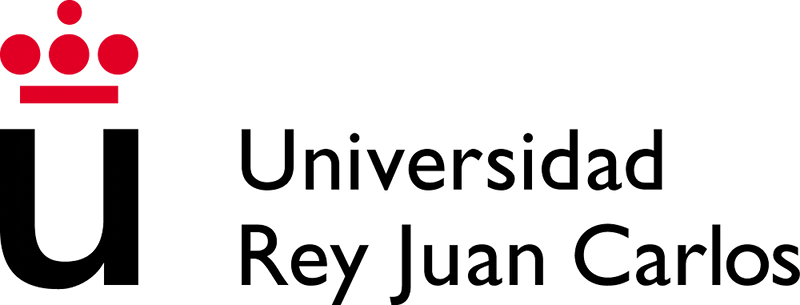
\includegraphics[width=0.6\textwidth]{logo}

		\vspace{1.5cm}
       \LARGE     
       Grado en ingeniería del software\\
       \Huge
       \textbf{Uso de blockchain como respaldo para el proceso KYC}
            
       \vspace{1.5cm}

		\Large
       \textbf{Autor: Christian Karem Taidi Santana}

       \vspace{3cm}  
       Resumen: El presente trabajo pretende proponer un sistema de intercambio de datos basado en la tecnología blockchain, asegurando la persistencia de la transacción, sin los datos, de forma permanente e inmutable, lo que permitiría tener un registro de los procesos de alta en un servicio para futuras consultas, sin riesgo de que pueda verse alterado o eliminado por error o de forma intencionada.
            
       \vspace{0.8cm}
     
       
       
       15/09/2020
            
   \end{center}
\end{titlepage}
\tableofcontents
\listoffigures




\chapter{Introducción y objetivos}
\section{Contexto}
Cada día en España se realizan procesos burocráticos para contratar servicios. Generalmente estos procesos son presenciales e involucran una cantidad elevada de trámites, firmas, documentos, intercambio de datos y en general tiempo, para cumplir con unos estándares estatales incluso mundiales correspondientes con la incorporación de clientes a un // sistema de cara a evitar fraudes fiscales, suplantaciones de identidad y falsificación de datos.

Éste proyecto pretende analizar el uso de la tecnología blockchain en el ámbito de la identidad digital y el intercambio de datos para el proceso de alta. Aprovechando sus cualidades y enfocandolo al problema de la persistencia de las transacciones de datos realizadas en dicho proceso sin vulnerar la confidencialidad ni el derecho al olvido del usuario por parte de los proveedores de servicio.

La tecnología blockchain nació en 2008 con el diseño teórico del protocolo Bitcoin, siendo en 2009 cuando se crearía la primera red Bitcoin real. Esta tecnología surgió como solución al problema del doble gasto que involucraba la duplicación y falsificación de modedas digitales, por la definición de la tecnología blockchain se soluciona este problema.

Aunque es una tecnología que nació para el ámbito económico, desde entonces se han buscado otros sectores en los que se podría aprovechar las cualidades de la blockchain tales como: El sector financiero, el sector sanitario, la ciberseguridad y el sector industrial.

En cuanto a la identidad digital, es un tema que a pesar de haber estado presente desde hace mucho tiempo, sigue teniendo problemas a la hora de gestionar datos identificativos ya que los modelos actuales para la persistencia y el intercambio de datos son los modelos centralizado y federado, haciendo que el usuario necesite de una tercera entidad para gestionar su información personal.
//
\section{Objetivo}
En este trabajo se propone determinar la utilidad de la tecnología blockchain como respaldo para los procesos de alta de usuario o Know Your Customer,// aprovechando sus características principales, y la eficiencia que otorga a todos los procesos correspondientes al alta de clientes en un sistema, tanto en recursos económicos como en tiempo. Para ello se necesitan conseguir los siguientes objetivos:

\begin{itemize}
\item Comprender el funcionamiento de la tecnología blockchain así como sus características.

\item Conocer las tecnologías asociadas al blockchain así como el contexto de su uso y su interacción.

\item Analizar las distintas implementaciones de la tecnología blockchain junto con sus ventajas y desventajas.

\item Comprender el funcionamiento de la identidad digital tanto en el ámbito de la ciberseguridad como en el de los servicios digitales.

\item Investigar casos de uso de la tecnología blockchain relacionados con la identidad digital.

\item Estudiar los mecanismos actuales para la gestión de identidades.

\item Investigar la regulación existente con respecto a la gestión de identidades y a la contratación de servicios.

\item Implementar un prototipo que sirva de ejemplo para un sistema de intercambio de datos que mantenga un registro del proceso KYC en una red blockchain.

\item Obtener unas conclusiones acerca del uso de la tecnología blockchain para registrar intercambios de datos y las ventajas y desventajas que esto conlleva.

\end{itemize}
//
\section{Planificación}
//
Este trabajo se ha planificado a largo plazo indicando una serie de hitos a completar para conseguir los objetivos. La planificación se muestra en el diagrama de Gantt de la Figura 1.1//
\begin{figure}[H]
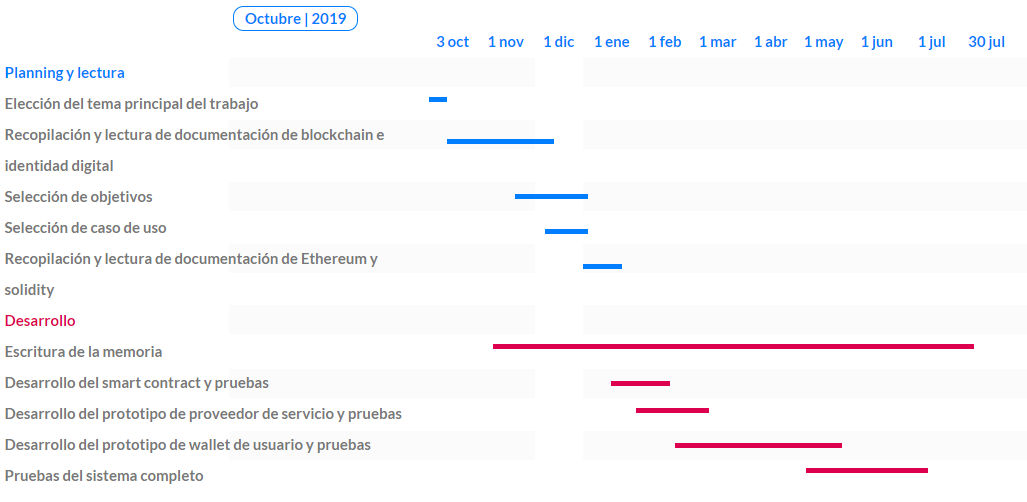
\includegraphics[width=1\textwidth]{Planning}
\caption{Planificación del trabajo}
\end{figure}
\section{Estructura}
El documento está organizado en 4 capítulos y un apartado de conclusiones. 

Capítulo 1: Introducción y objetivos (Este capítulo).

Capítulo 2: Identidad digital y Blockchain.
En éste capítulo se hace una breve explicación del concepto de identidad digital, los distintos tipos que existen, para qué sirve y los aspectos legales que conllevan la utilización de una identidad digital.
Además se introduce la tecnología blockchain explicando los tipos de blockchain, la estructura y se concreta un poco más en Ethereum que será la blockchain utilizada en el caso de uso.

Capítulo 3: Casos de Uso.
En éste capítulo se explican varios casos de uso de la tecnología blockchain relacionado con la identidad digital, como puede ser el proceso Know Your Customer y Self Sovereign Identity.


Capítulo 4: Caso de uso: Alta en la universidad con registro del proceso KYC en Ethereum.
En este capítulo se desarrollará el caso de uso del trabajo.

Conclusiones.
En éste apartado se incluyen todas las conclusiones a las que se ha llegado mediante la realización del trabajo, problemas encontrados y decisiones tomadas con su razón.

\section{Terminología}
\begin{itemize}

\item
Entidad: Objeto físico o lógico que tiene una existencia distintiva sea de forma física o lógica. 
Esta existencia se puede medir en base a diferentes atributos.
En el contexto de éste trabajo nos enfocaremos a entidades digitales que son simplemente una representación digital de una entidad y se asume que una entidad digital es una persona o bien una organzación que provee de algún servicio online 

\item
Assert: Objeto lógico otorgado a una entidad que le da unas propiedades determinadas, generalmente son objetos identificativos, certificados, y documentos oficiales asignados a una identidad física para asignarle una serie de cualidades.

//
\item
Asset: Activo de un usuario que puede ser una criptomoneda o bien acciones de una empresa. En el contexto de este trabajo serán las criptomonedas que posea un usuario en su cartera digital y que usará para realizar transacciones.

\item 
Attester: Entidad de confianza encargada de certificar y otorgar asserts a los usuarios, además de garantizar la exactitud con la realidad de dichos asserts.

\item
CA(Certificate Authority): Entidad de confianza responsable de emitir y revoccar certificados firmados electrónicamente.
//
\item
TTP (Third Trusted Party): Entidad en la que confian otras entidades en un entorno concreto.
Una TTP se aprovecha para generar Asserts sobre una entidad que serán fiables para otras entidades.

\item
Claim: Un claim es una afirmacion acerca de una entidad, consiste en un atributo de par clave-valor (tambien puede ser una colección de varios atributos). Dicho claim puede ser generado por la misma entidad o por una TTP.

\item
Credencial: Elemento identificativo que relaciona una entidad física con una entidad lógica o digital. Asegura que al utilizar una entidad lógica para cualquier trámite, esta se corresponde con una persona física.

//
\item
Faucet: Sistema de recomensa que premia con criptomonedas a los usuarios de una red blockchain por completar tareas como resolver un captcha o cualquier otro tipo de tarea.

\item
Wallet: Dispositivo, medio físico, programa o servicio que almacena las claves pública y privada de una cuenta en una red blockchain, y que pueden utilizarse para realizar transacciones de criptomonedas o trazar las posesiones de una entidad. La clave pública permite a las demas wallets realizar pagos a la dirección de la cartera, mientras que la clave privada se utiliza para gastar criptomodedas desde la cuenta a la que pertenece.

\item
Hash: Puede decirse de la función que transforma un bloque arbitrario de datos en una serie de caracteres con longitud fija. O bien la serie de caracteres resultantes de aplicar la función hash a un bloque de datos.
//
\end{itemize}
\chapter{Identidad digital y blockchain}
\section{Identidad digital}

La identidad digital es la representación de un individuo que está involucrado en una transacción online. Una identidad digital es única en el contexto de un servicio digital, pero no necesariamente identifica al sujeto en todos los contextos, una misma persona puede tener una cuenta de correo electrónico, una cuenta en algún videojuego online, un identificador en una red peer-to-peer para realizar intercambio de datos. La persona es la misma pero para cada servicio utiliza un identificador distinto; es decir identificar a un sujeto en un servicio online no necesariamente equivale a identificar utilizando una identidad real. Peter Steiner en The New Yorker, “On the internet, nobody knows you’re a dog.” \cite{steiner1993internet} 
//
Para ello se establecen dos pruebas para verificar una identidad digital.
La prueba de identidad establece que un individuo es quien afirma ser.
La autenticación establece que un individuo que desea acceder a un servicio, posee uno o varios autenticadores válidos asociados con la identidad del mismo.
//
La identidad digital presenta un problema técnico ya que las pruebas de identidad se suelen llevar a cabo y siempre involucran, un proceso de autenticación sobre una red abierta, para acceder a servicios gubernamentales digitales. Los procesos y tecnologías establecidos para usar identidades digitales ofrecen muchas oportunidades para suplantaciones y otros ataques.

Dicha identidad se suele representar como una serie de letras y números denominada clave pública, ésta clave es conocida por todo el mundo y es la que se usará para comunicarse de forma segura con el individuo.

//
Se requiere un proceso de autenticación de usuario. 
Esto genera varios problemas y varias necesidades, como la capacidad de utilizar un identificador universal para todos los servicios digitales y que dicho identificador se corresponda con una única persona real de forma bidireccional. Al no tener un protocolo común es necesario hacer transacciónes de datos físicos para identificar a un individuo en un servicio de forma real lo que conlleva un proceso burocrático generalmente lento.
//

\subsection{Tipos de identidad digital}

\begin{itemize}
\item {\textbf{Identidad Centralizada:}}
Utilizada generalmente en los servicios digitales, se basa en la creación de una identidad en el servicio consistente generalmente en un usuario y una contraseña. Por ejemplo una cuenta de correo electrónico gmail, se puede utilizar como identificador en varios servicios pero tu identidad está almacenada en los servidores de google y la relación con los distintos servicios en los que se utilize como identificación.

\item {\textbf{Identidad Federada:}}
Este modelo de identidad necesita una tercera parte que se encargue de otorgar un assert al usuario de forma que los distintos servicios en los que el usuario quiera darse de alta contrastará la información proporcionada con el proveedor de identidad, es equivalente a un TTP. De esta forma el usuario no necesita generar unas credenciales nuevas cuando se da de alta en un servicio sino que puede utilizar la emitida por esta entidad, ya que será de confianza para el servicio.
 
\item{\textbf{SSI Self Sovereign Identity:}}
Consiste en un modelo de identificación entre un usuario y un proveedor de servicio sin necesidad de un intermediario, de esta forma el usuario puede gestionar sus datos identificativos en lugar de dejar a una entidad externa ser propietaria de dichos datos, y que pueda usarlos o venderlos a empresas de publicidad sin consentimiento del usuario.

\end{itemize}

\subsection{Autenticación y Verificación}

La autenticación y la verificación son dos procesos ligados al uso de una identidad digital que permiten añadir control de acceso y de permisos en un servicio, lo que añade una capa de confidencialidad e integridad a los activos asociados a una identidad.

\subsection{Autenticación}

El proceso de autenticación consiste en la demostración por parte del usuario de poseer un autenticador que está ligado a la identidad que se quiere utilizar mediante un protocolo de autenticación.

Ésta interacción entre el verificador y el usuario es extremadamente importante a la hora de determinar la seguridad del sistema, ya que un protocolo bien diseñado puede proteger la integridad y la confidencialidad de la comunicación entre ambos durante y después de la autenticación, y puede ayudar a limitar el daño hecho por un atacante suplantando al verificador legítimo.

Además el sistema verificador puede mitigar ataques de adivinación contra claves secretas con baja entropía, limitando el número de intentos de autenticación.

\subsection{Verificación}

El proceso de verificación consiste en determinar si una identidad digital corresponde con el individuo que dice poseer dicha identidad, lo que enlaza en más profundidad a un individuo con la información que suministra. En este proceso se intenta verificar que los datos introducidos son reales haciendo comprobaciones con bases de datos oficiales o confiando en que los datos iniciales son legítimos y contrastando con estos. Éste procedimiento suele hacerse en servicios a los que se les exige demostrar que sus clientes existen realmente (por ejemplo un banco), para esto se suelen tener en cuenta tres factores:

\begin{itemize}
\item
Algo que sepa: Por ejemplo una contraseña, un pin, un dato...
\item
Algo que tenga: Un dispositivo asignado a el, una tarjeta de teléfono, un ordenador...
\item
Algo que sea: Un dato biométrico del individuo ya sea la huella, el iris, la cara, una muestra de sangre...
\end{itemize}

\subsection{Aspectos legales}

La identidad física se asocia a una serie de características de cada persona, desde el nombre, la edad, el género, gustos y/o preferencias etc...

La identidad digital intenta conseguir el mismo nivel de información correspondiente al mundo físico pero publicada a través de internet y complementada con otros elementos como el correo electrónico o la firma digital. Aunque esto son elementos privados, permiten a los usuarios autorizados o a terceras partes el acceso a datos personales que identifican a un individuo en el mundo físico. 
Por ejemplo Signaturit ofrece la posibilidad de que terceras partes u otras partes interesadas validen la identidad de las partes involucradas en la firma de un documento.

La identidad digital no tiene reconocimiento legal pero los derechos asociados a la identidad física se extienden a la digital y por tanto son aplicables a esta. Estos derechos son los decretados en la Declaración Universal de Derechos Humanos de forma internacional y en España, en la constitución y la ley orgánica.






\section{Introducción a Blockchain}

La tecnología blockchain se considera un historial/registro, distribuido, descentralizado y permanente, de transacciones o hechos ocurridos en cierto momento.
En todo momento se certifica que los datos contenidos en él no han sido modificados tras haber sido incluidos.
\begin{figure}[h]

\includegraphics[scale=0.3]{ledger}
\caption{Libro de cuentas}
\end{figure}

Las transacciones realizadas a traves del sistema se llevan a cabo entre las partes de forma directa sin necesidad de un intermediario ya que, al asegurar en todo momento la persistencia de los datos representativos de la transacción y la inmutabilidad de los mismos, no es necesario que verifique que la transacción sea correcta, pues esto se realiza en consenso por todos los nodos que forman la red. Esto agiliza el proceso a la hora de realizar dichas transacciones y además reduce el coste económico al no necesitar de una autoridad central que almacene estos datos.

Se considera distribuida porque la información contenida en la cadena no está persistida en un servidor central, sino que está replicada entre todos los nodos de la red, asegurando no solo la persistencia sino la disponibilidad de la misma.

Es descentralizada porque el poder de cómputo se reparte entre todos los nodos conectados a una red peer-to-peer en lugar de depender de un servidor central.
\begin{figure}[h]
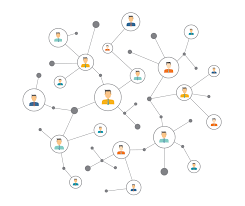
\includegraphics[scale=0.7]{network}
\caption{Red peer-to-peer}
\centering
\end{figure}

Es inmutable porque en el momento en que se añade un bloque a la cadena, éste no puede ser modificado sin corromper la cadena haciendo que sea inválida, ya que los bloques están criptográficamente enlazados entre sí.

\begin{figure}[h]
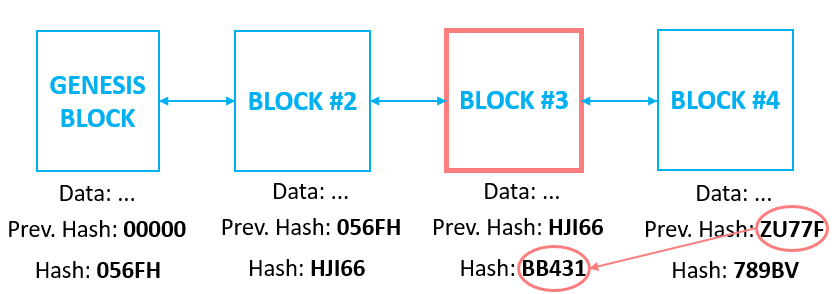
\includegraphics[scale=0.5]{immutable}
\caption{Fallo de enlace criptográfico entre bloques}
\centering
\end{figure}

El pilar principal de la seguridad que se cumple en blockchain es la integridad ya que al ser inmutable, la información no puede ser modificada por nadie. Esto es debido a que es un registro distribuido y a los protocolos de consenso para validar la inserción de un bloque en la cadena.

Aunque no está implícito en la definición de blockchain, se puede añadir una capa de criptografía que asegure la privacidad de cada participante mediante un mecanismo de clave asimétrica, pudiendo así verificar que los datos de una transacción pertenecen a un usuario debido a que se ha añadido su clave pública a la transacción a modo de firma sin revelar en ningún momento sus datos. Éste par de claves pública/privada suele estar asociado a un wallet al que accede el usuario para gestionar sus transacciones a través de la red.



Además de esto, el código fuente suele ser OpenSource por lo que todo el mundo puede examinar el código en caso de no confiar en el algoritmo usado o el protocolo de consenso.

\subsection{Tipos de blockchain}
Existen dos tipos de blockchain dependiendo de cómo se incorporan los nodos a la red, y la capacidad de actuación que tiene cada uno en el sistema.

\begin{itemize}


\item \textbf{Blockchain sin permisos (Ejemplo: Bitcoin, Ethereum):} 
Cualquiera puede ser un usuario o llevar un nodo, cualquier persona puede escribir en la cadena realizando transacciones, y cualquiera puede participar en el proceso de consenso para determinar la validez de un estado.
Los nodos registrados en ésta blockchain participan de forma anónima o pseudoanónima y suelen funcionar con el algoritmo de Proof Of Work como incentivo para que los nodos participen en la red.

\item \textbf{Blockchain con permisos:} 
Está gestionada por una entidad conocida en la que miembros de un consorcio operan en dicha cadena.
Los nodos se identifican de forma no anónima para poder participar y cada nodo puede tener un rol específico asignado relacionado con los permisos otorgados.
Dependiendo de la distribución de dichos permisos se derivan dos tipos de blockchain con permisos.

\begin{itemize}
\item
\textbf{Blockchain Pública:}
Todos los participantes tienen la capacidad de leer y verificar la consistencia de la cadena permitiendo una descentralización de la computación aunque la blockchain esté gobernada por un consorcio.
\item
\textbf{Blockchain Privada:}
Sólo un número concreto de nodos puede leer y verificar las transacciones almacenadas de forma que se centraliza el consenso en un grupo pequeño.
\end{itemize}

\end{itemize}
\subsection{Estructura}

\begin{itemize}


\item

	Bloque: El componente principal de la blockchain son los bloques, que representan una unidad de información enlazada a otros bloques criptográficamente, esta información suele ser transacciones entre individuos o información adicional que se quiere certificar.
	La forma de añadir un bloque a la cadena depende de los algoritmos de consenso y de la implementación concreta de la cadena.
	
\item

	Cadena: Conjunto de bloques enlazados mediante la inclusión de un valor en cada bloque que representa el valor hash del bloque anterior, gracias a esto, es imposible alterar la información de un bloque sin corromper la estructura de la cadena.
	Éste hash se forma teniendo en cuenta varios campos de información del bloque, principalmente los datos que contiene, el sello de tiempo en el que se generó el bloque y el hash del bloque anterior.
\begin{figure}[h]
	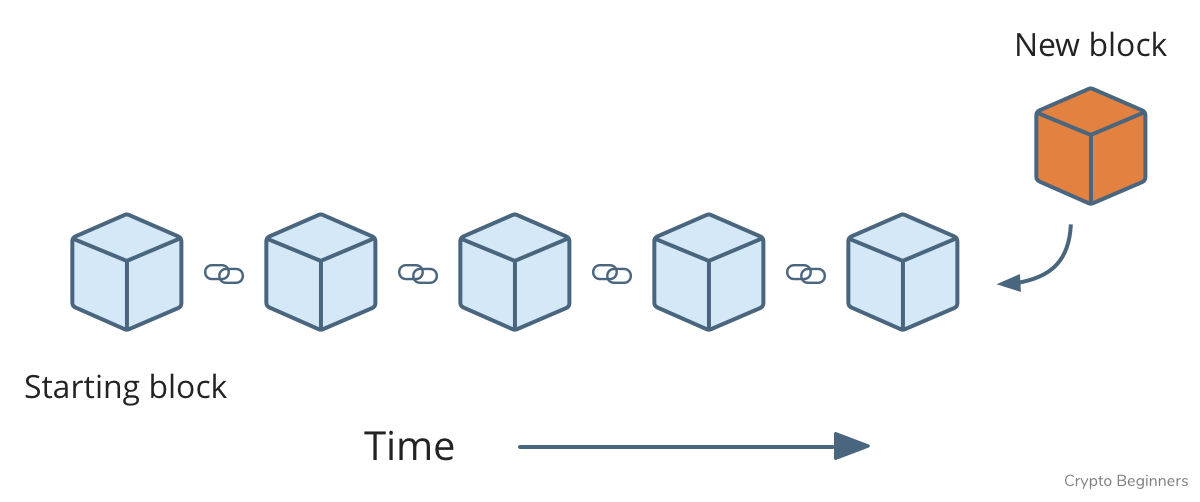
\includegraphics[scale=0.4]{new-block}
	\caption{Cadena de bloques ligados criptográficamente}
\end{figure}
\item

	Nodos: Conjunto de individuos o máquinas conectadas a la red P2P blockchain que se dedican a añadir transacciones, construir bloques, validar cadenas y distribuir la cadena.
	Todos estos nodos actuan de acuerdo a un protocolo de consenso implícito en el código de la cadena de forma que ninguno tiene capacidad de corromper la cadena.
\end{itemize}	
\subsection{Protocolo}

	Protocolo de red que utilizan los nodos para comunicarse entre sí produciendo la distribución de la cadena, de forma que todos tengan una forma común para compartir información.
	

	
	
\subsection{Algoritmos de consenso}

	Algoritmo usado para, en caso de generar dos bloques simultaneos antes de ser distribuidos, elegir qué bloque se añadirá primero a la cadena principal, y en caso de generarse varias subcadenas, elegir cual persistirá en la red.
	En el ámbito del blockchain, existen cuatro modelos de consenso principales:
\begin{figure}[h]
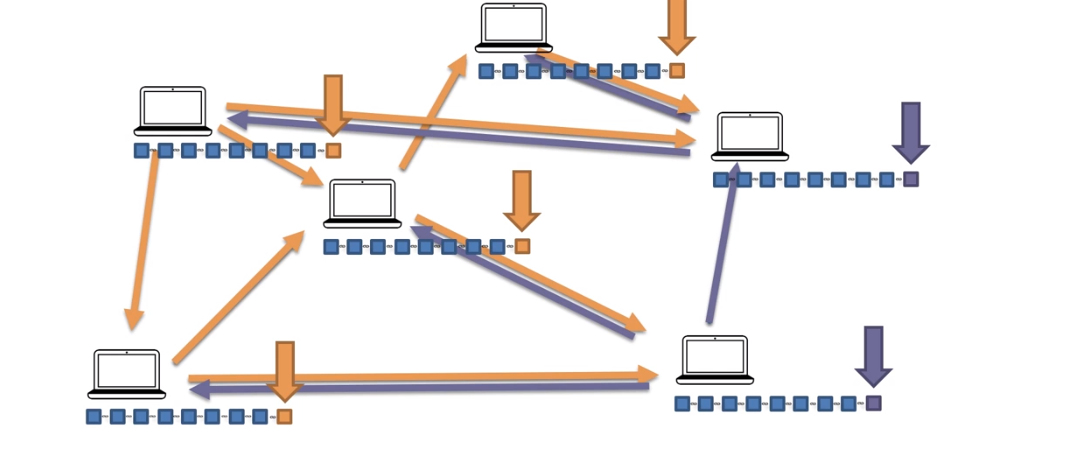
\includegraphics[scale=0.5]{consenso}
\caption{Selección de cadena más larga}
\end{figure}
	
\begin{itemize}
\item Proof of Work (PoW)

	Mecanismo de consenso que detecta ataques de denegación de servicio o spam en una red haciendo que se requiera trabajo computacional del emisor de la petición de forma que tome un tiempo realizarla.
	 
	 Una característica clave de este esquema es su asimetría. el trabajo realizado por el emisor de la petición debe ser moderadamente alto mientras que el proveedor de servicio debe poder comprobar fácilmente que se ha realizado el trabajo, se conoce como función de coste de CPU o puzle computacional.
	  
\item Proof of Stake (PoS) 

	Algoritmo de consenso para redes distribuidas que asegura una red blockchain mediante la petición de pruebas de posesión de criptomonedas.
	
	La probabilidad de encontrar un bloque de transacción y recibir el premio es proporcional a la cantidad de criptomonedas acumuladas de cada entidad. De esta forma la confianza no se basa en el trabajo computacional realizado, sino en la suposición de que la entidad con más monedas es la más interesada en la supervivencia de la red, por tanto se les premia con menor dificultad para encontrar bloques ya que estos deberían tener más poder de consenso en la red.
	
\item Proof of Authority (PoA)

	En este algoritmo de consenso, las entidades son premiadas en base a su reputación ya que los verificadores de la red añaden su identidad real de forma que se demuestre transparencia por su parte, por esto suele haber un número limitado de validadores elegidos de forma aleatoria. Estos validadores deben revelar su identidad de forma voluntaria, así cuidarán de su identidad y reputación y por esa razón, velarán por el buen funcionamiento, la transparencia y fiabilidad de la operación de la misma.
	
	Este protocolo suele estar orientado a blockchain de tipo privada de forma que solo ciertos nodos con permiso pueden participar.

\item Proof of Capacity (PoC)

	Este algoritmo de consenso es muy parecido al PoW salvo que en lugar de determinar el interés de una entidad por su capacidad computacional, se determina por capacidad de memoria, asignando una candidad de memoria, o espacio en disco, no trivial, para resolver un reto presentado por el proveedor de servicios.
	
	Se presenta como una alternativa al PoW ya que se entiende que PoC es más justo y ecológico, ya que el almacenamiento suele tener un propósito genérico y tiene un menor coste energético.
	
\end{itemize}	 
\subsection{Dificultad}

	La dificultad de una blockchain suele utilizarse para definir el tiempo que debe pasar entre la incorporación de un bloque a la cadena, y la incorporación del siguiente, ésto se suele ajustar añadiendo un requisito al hash de cada bloque de forma que cada máquina que quiera añadir un bloque nuevo necesite un tiempo de computación que se acerque al requerido por la cadena.
	
\subsection{Criptografía}

\begin{itemize}


\item Criptografía de bloque:

Cada bloque de la cadena se genera obteniendo un código hash en base a ciertos campos contenidos en el bloque.
Para obtener éste código hash se suele utilizar la función SHA256 que genera un código de 64 cifras hexadecimales representando una información de tamaño variable.

	Ésta función hash tiene una serie de requisitos:
	
	\begin{itemize}
		\item La salida debe ser siempre del mismo tamaño.
		
		\item La entrada puede ser de tamaño variable.
		
		\item Dada una función hash $H$, $H(X)$ debe ser fácilmente computable para cualquier $x$. 	
		
		\item La función $H$ debe ser unidireccional, es decir, dado un hash $h$ es computacionalmente infactible encontrar una entrada $x$ tal que $H(x)=h$.	
		
		\item La función $H$ debe ser débilmente resistente a colisiones, es decir, dado un valor $x$ es computacionalmente infactible encontrar un valor $y$ tal que $H(x) = H(y)$.
		
		\item La función $H$ debe ser fuertemente resistente a colisiones, es decir, debe ser computacionalmente infactible encontrar dos valores $x , y$ cuales sea tal que $H(x) = H(y)$.
		
	\end{itemize}
		
	Estos requisitos son esenciales en la tecnología blockchain ya que si se incumpliese alguno, o bien sería demasiado costoso obtener el hash de un bloque, o bien se podría alterar los datos de un bloque aprovechando una colisión en su hash, modificando así los datos del mismo sin que cambie su ``huella".

\item Firma digital:

Se utiliza un sistema de criptografía asimétrico para proporcionar un mecanismo de firma digital a la hora de certificar identidades.
\begin{figure}
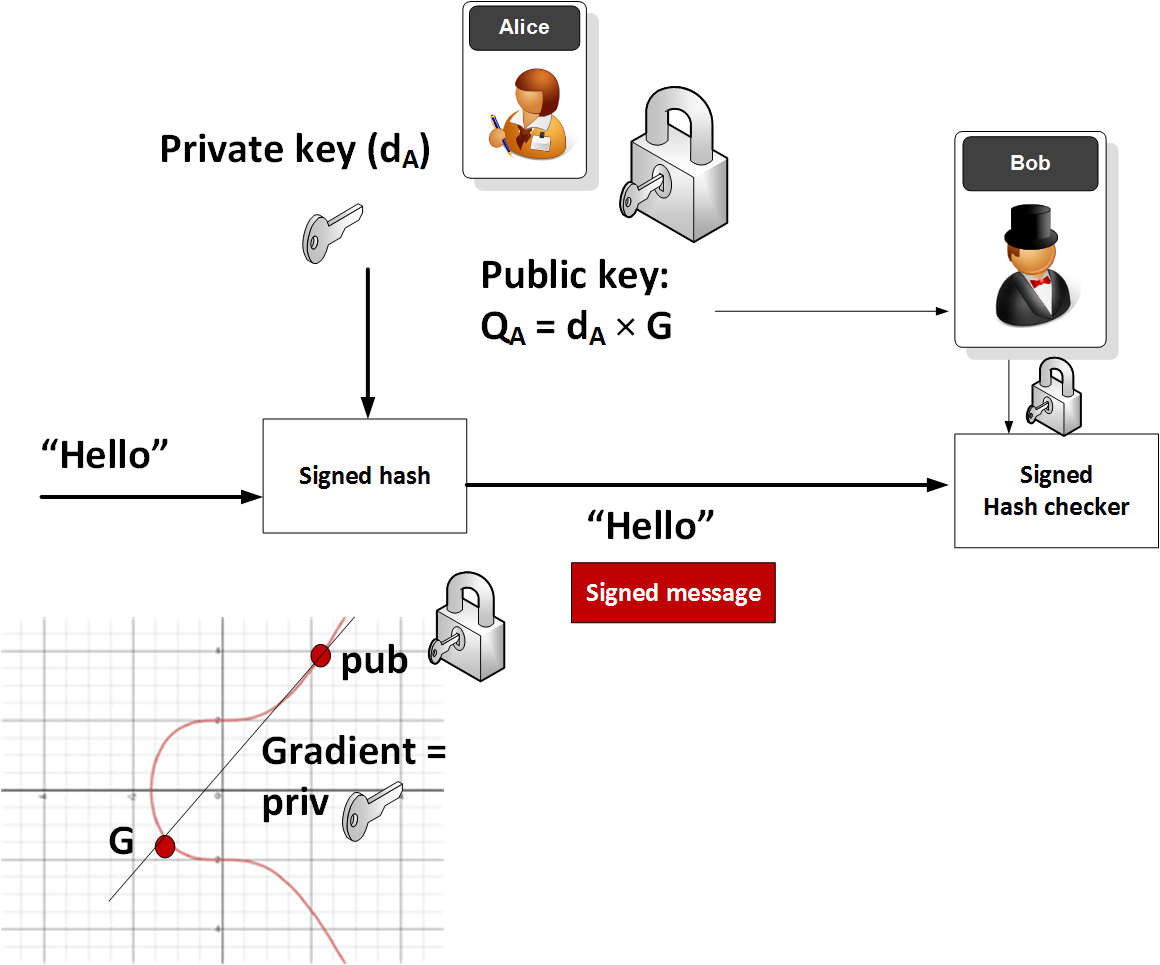
\includegraphics[scale=0.3]{digital-sign}
\caption{Firma digital mediante uso de claves asimétricas}
\end{figure}

Para generar tanto la clave pública como la privada se suele utilizar una curva elíptica ECDSA (Elliptic Curve Digital Signature Algorithm) ya que el tamaño de las claves es más pequeño reduciendo así requisitos de almacenamiento y transmisión. La criptografía basada en curvas elípticas puede dar el mismo nivel de seguridad con una clave de 256 bits que RSA (Rivest, Shamir y Adleman) con 2048 bits, de esta forma se facilita el manejo de direcciónes públicas.

Para hacer que sea más ligera se suele aplicar también una función hash a las claves, haciendo que todas tengan un tamaño fijo.
\end{itemize}
\subsection{Wallet}

Un Wallet no es más que una billetera virtual en la que el usuario puede gestionar sus activos relativos a la blockchain, generalmente esos activos son criptomonedas pero en el caso que nos concierne los activos serán datos del usuario denominados Asserts.

\section{Ethereum}
Ethereum es una blockchain programable que se lanzó en 2005 y actualmente es la líder en éste tipo de blockchains.
Como todas las blockchains, tiene una criptomoneda (ETH) que funciona igual que cualquier otra criptomoneda, pudiendo enviarse a cualquier persona de forma instantánea.

A diferencia de muchas otras blockchains es programable, lo que significa que los desarrolladores pueden usarla para desarrollar nuevos tipos de aplicación conocidas como DAPPs (Decentralized Applications) que adquieren los beneficios de las criptomonedas y la tecnología blockchain, estas aplicaciones son fiables ya que una vez se desplieguen a la red, funcionaran tal y como se han programado. Se pueden emplear para gestionar assets digitales para crear nuevos tipos de aplicaciones financieras, y pueden ser descentralizadas lo que significa que ninguna entidad o persona controla esta aplicación. Actualmente los desarrolladores están construyendo aplicaciones descentralizadas como carteras de criptomonedas, aplicaciones financieras, mercados descentralizados, juegos y mucho mas.

No hay ninguna compañia u organización central que controle la red ethereum, está mantenida y mejorada por una comunidad global de contribuyentes que trabajan desde el protocolo principal hasta aplicaciones de consumidor.

\subsection{Smart Contract}

A lo largo de los años el concepto de Smart Contract se ha utilizado para describir multitud de cosas. En los 90 el criptógrafo Nick Szabo acuñó el término para enfatizar el objetivo de llevar las prácticas de la ley de contratos y las prácticas comerciales relacionadas hacia el diseño de protocolos de comercio electrónico entre desconocidos a través de internet.

En el contexto de Ethereum el término está equivocado ya que los Smart Contract en Ethereum no son ni un contrato legal ni inteligentes, pero el término se ha quedado. En este contexto por tanto se refiere a Smart Contract como un programa inmutable que se ejecuta de forma determinista en el contexto de una máquina virtual de Ethereum o EVM como parte del protocolo de red Ethereum de forma descentralizada.
Las características que definen a un smart contract son las siguientes:

\begin{itemize}
\item Programa: Un smart contract es simplemente un tipo de programa ejecutado en la EVM, el término contrato no tiene ningún significado legal en éste contexto.
\item Inmutable: Una vez desplegado, el programa no se puede modificar a diferencia del software tradicional, la única forma de modificar un smart contract es desplegar una instancia nueva con las modificaciones necesarias.
\item Determinista: La salida de la ejecución de un smart contract es la misma para cualquiera que lo ejecute dado el contexto de la transacción que ha iniciado la ejecución y el estado de la blockchain Ethereum en el momento de la ejecución.
\item EVM: Los smart contract se ejecutan en un contexto muy limitado, pueden acceder a su estado, al contexto de la transacción que lo ejecuta y a alguna información de los bloques más recientes.
\end{itemize}
\subsection{Ciclo de vida}
Los smart contract se escriben en lenguaje de alto nivel, generalmente Solidity, pero para ejecutarlos deben ser compilados en el bytecode utilizado por la EVM. Una vez compilado se despliega en la blockchain utilizando una transacción especial para crear contratos. Cada contrato se identifica con una dirección Ethereum que está derivada de la transacción de creación del contrato como una función de la cuenta que lo ha creado y el nonce, que consiste en un valor calculado a la hora de resolver el puzle critográfico del bloque y definido por la dificultad de la red para generar dicho bloque.

La dirección del contrato se puede utilizar en una transacción como el receptor para enviar fondos al smart contract o para llamar a una función del mismo.

A diferencia de las cuentas de Ethereum, los smart contracts no tienen claves asociadas a las cuentas creadas para estos (al usar una dirección ethereum, se entiende que se crea una cuenta), y como creador del contrato no se te otorga ningún privilegio especial a nivel de protocolo. Esto junto con la no-existencia de una clave privada, se puede decir que un smart contract se pertenece a si mismo una vez está desplegado.

Un smart contract solo se ejecuta si es llamado a partir de una transacción inciada por una cuenta poseida externamente EOA (Externally owned account) o cuenta de usuario. Los smart contract pueden invocar funciones de otro smart contract de forma sucesiva, pero la llamada al primer smart contract tendrá siempre como origen una transacción iniciada por una EOA, por tanto no se ejecutan a si mismos ni en segundo plano, se encuentran a la espera de que se llame a alguna función a partir de una transacción. Tampoco se ejecutan en paralelo las funciones del smart contract, se entiende que el ``Ordenador mundial de Ethereum'' es una máquina monohilo.

Todas las interacciones con un smart contract, sea para desplegar o invocar una función, tienen un coste en gas para el usuario que realiza dicha interacción. Este coste pretende limitar el despliegue y uso de funciones de smart contract para evitar inundaciones y colapso de la red.

Las transacciones realizadas a partir de un smart contract son atómicas es decir, si surge algún tipo de fallo durante la ejecución de una transacción, todos los cambios son revertidos al estado original aunque se queda registrada como un intento fallido de transacción en la blockchain.

\chapter{Casos de uso de blockchain e identidad digital}

\section{Proceso KYC (Know Your Customer)}

En el momento en que un usuario decide darse de alta en un servicio, este solicita una serie de datos identificativos para saber quién va a ser su usuario/cliente. Pongamos el ejemplo de la Universidad Rey Juan Carlos, cuando una persona decide matricularse digamos en un plan de estudios de grado, la universidad solicita una serie de datos identificativos y certificados, ya que se deben cumplir una serie de condiciones en una persona que quiera cursar un grado (nota de selectividad si se entra por prueba de acceso, certificado de estudios anteriores si se han realizado estudios previos de grado etc). Estos datos es necesario que se obtengan con el consentimiento del usuario y quede registrado el intercambio de alguna forma para posteriores consultas.



\subsection{Motivación}

Éste proceso es importante para las actividades administrativas de los distintos proveedores de servicio, ya que generalmente deben dar explicaciones y tener un respaldo que justifique el hecho de que una persona esté dada de alta en su sistema. Si ésto no fuese así, cualquier proveedor de servicio podría alegar que un individuo ha sido dado de alta en su sistema sin que éste en ningún momento haya compartido sus datos con la identidad ni siquiera haya dado su consentimiento para que tenga los datos o para que figure su alta en el sistema.
Pongamos por ejemplo el alta en una entidad bancaria con un servicio que tiene un coste de mantenimiento y de comisión de apertura ligado al usuario. Si la entidad bancaria por algún motivo decide dar de alta a un usuario y hacer cobros relacionados con los servicios que afirman que el usuario ha solicitado, éste puede negarlo facilmente gracias a este proceso ya que la entidad bancaria no puede demostrar que haya obtenido datos ni consentimiento del usuario.

Este concepto suele aplicarse principalmente a entornos financieros, para evitar que se utilicen los bancos como medio para el blanqueo de capitales. Al pasar el proceso, se pretende conocer con exactitud al cliente analizando sus datos personales y sus movimientos bancarios, para así crear unas expectativas y predecir el comportamiento transaccional en un futuro.

Pero se puede aplicar a cualquier contexto y a cualquier servicio, ya que en todos los casos en los que se ofrezca un servicio a un cliente se necesita conocer quién es, no solo para evitar fraudes sino para ofrecer una atención adecuada y personalizada.

\subsection{Soluciones}

La solución que se tiene en cuenta actualmente es llevar un registro de dichos datos certificados, sellados y/o firmados relacionados con dicho usuario, junto con una firma del usuario que asegura el consentimiento. Todo esto conlleva un proceso burocrático largo en el que el usuario debe pedir a las entidades pertinentes sus datos identificativos solicitados por el proveedor de servicio. Posteriormente el usuario deberá acudir al proveedor de servicio con los datos y firmar el consentimiento. Por parte del proveedor de servicio, tiene que encargarse de asegurar la persistencia tanto de los datos asociados al usuario como de su consentimiento para futuras consultas. Puede ser de forma física (archivado en papel) o digital (base de datos de clientes) ambos tienen riesgo de pérdida, modificación y exposición, (el papel se puede quemar, alterar, robar ... , y la base de datos puede sufrir una fuga de datos, puede perderse información o puede surfrir modificaciones no autorizadas).

Hay una solución que es la que se propone en éste trabajo que utiliza únicamente medios digitales y se asegura la confidencialidad, la persistencia y la inmutabilidad. Consiste en registrar éste proceso de intercambio de datos como una transacción blockchain de forma que se pueda demostrar sin necesidad de almacenar los datos en la cadena, que efectivamente se ha cumplido el proceso KYC entre un usuario y un proveedor de servicio.

Ésto además puede combinarse con el concepto de wallet e identidad auto-soberana, de forma que se evite el proceso burocrático mencionado anteriormente, ya que el usuario poseerá en todo momento en su wallet los assert otorgados por los diferentes attesters. En el momento de querer darse de alta en un servicio, simplemente compartirá los assert necesarios con el proveedor a traves de un smart contract desplegado en una red Ethereum con el fin de mantener registradas las interacciones con el contrato que serán equivalentes al proceso KYC. 

\section{Self Sovereign Identity SSI}
Como se ha mencionado anteriormente existe un tipo de identidad digital conocidad como Self Sovereign Identity que consiste en una identidad gestionada por el propio individuo al que identifica, lo que le otorga el poder de elegir a quién y cómo facilita sus datos identificativos sin necesidad de un intermediario.

\subsection{Motivación}
Este tipo de identidad permite una mayor eficiencia a la hora de almacenar y validar datos identificativos de un individuo. Permite al usuario tener control sobre sus datos sin necesitar de una entidad gubernamental o de consorcio que los gestione, almacene y proteja, por tanto el propio usuario puede utilizar sus datos de forma autónoma y acceder a ellos cuando lo necesite.

Al disponer de un registro inmutable, distribuido y que garantiza el no repudio, se asegura que el usuario siempre tendrá acceso a sus datos, que estos datos son los que se almacenaron en un principio, y que los datos no se perderan ya que se encuentran duplicados en miles de máquinas que actúan como base de datos distribuida.

\subsection{Problemas}
Se propone utilzar una blockchain como almacén inmutable de estos datos identificativos de forma que se pueda validar facilmente si una identidad es verdadera en base al hash generedo por el bloque que contiene estos datos. Pero tras la vigencia de la RGPD (Regla General de Protección de Datos) que otorga a cualquier individuo el derecho al olvido de todos los datos que se haya proporcionado, al ser la blockchain inmutable no es posible eliminar de la cadena los datos incorporados asociados al individuo que quiera recurrir a su derecho, por tanto se incumpliría esta norma.
//
Aunque los asserts estén almacenados en la blockchain, y el usuario sea propietario único de dichos datos, se necesita siempre una entidad de certificación encargada de otorgar esos asserts al usuario, firmados y certificados. Por ello el usuario no tendrá el poder de generar sus propios asserts válidos para cualquier proveedor de servicio, si esto no fuese así cualquier usuario podría falsificar sus datos. Esto implica que el usuario siempre va a depender de una tercera parte, para obtener sus datos identificativos oficiales, en la que confien los proveedores de servicio que quiera contratar.//
\subsection{Soluciones}
//
Para subsanar el problema del incumplimiento de la ley se podría incorporar una base de datos alternativa que asociase datos a un hash. en lugar de almacenar los datos identificativos en la cadena lo que convertiría a la blockchain en una lista de punteros a datos almacenados en dicha base de datos. Al aplicar esta solución se pierde la cualidad de auto-soberanía, pues los datos de usuario están almacenados en una base de datos que muy probablemente esté gestionada por un consorcio o una entidad externa al usuario, y la blockchain actuaría únicamente como comprobante para asegurar que los datos a los que se apunta, son los correspondientes al hash almacenado en la cadena.
//
\chapter{Caso de uso: Alta en la universidad con registro del proceso KYC en Ethereum}
En este capítulo se propone un caso de uso como ejemplo del uso de la tecnología blockchain para el registro del proceso KYC. Para esto se analizará la motivación, el funcionamiento básico y la arquitectura y requisitos necesarios para poder desarrollar el prototipo.

\section{Motivación}
Darse de alta en cualquier sistema o servicio suele requerir un proceso burocrático complejo que involucra solicitar múltiples datos certificados, conservarlos y transmitirlos, lo que suele ser un proceso lento y tedioso tanto para el usuario como para el servicio que solicita. Además este proceso necesita ser almacenado por el service provider ya que debe tener una forma de demostrar que se ha realizado el proceso de solicitud de datos al usuario y el consentimiento del mismo a la hora de compartirlos. Al hacerse este proceso de forma física principalmente, supone aún más coste en tiempo para el proveedor de servicio ya que deberá almacenar todos los documentos relevantes de forma indefinida para poder demostrar en un futuro que se ha encargado de solicitar, verificar y validar los datos identificativos de todos sus usuarios.

\section{Elementos}
En el prototipo hay 4 elementos principales: un CA encargado de otorgar los asserts a los usuarios, en este caso el DNI, un proveedor de servicio que solicitará una serie de datos identificativos al usuario, en este caso será la universidad, un usuario que será el que solicita darse de alta en el servicio y que recibirá y almacenará los asserts en su wallet, la red blockchain utilizada para desplegar el smart contract y realizar las transacciones, y un smart contract desplegado para registrar todo el proceso de intercambio de datos.
\begin{figure}
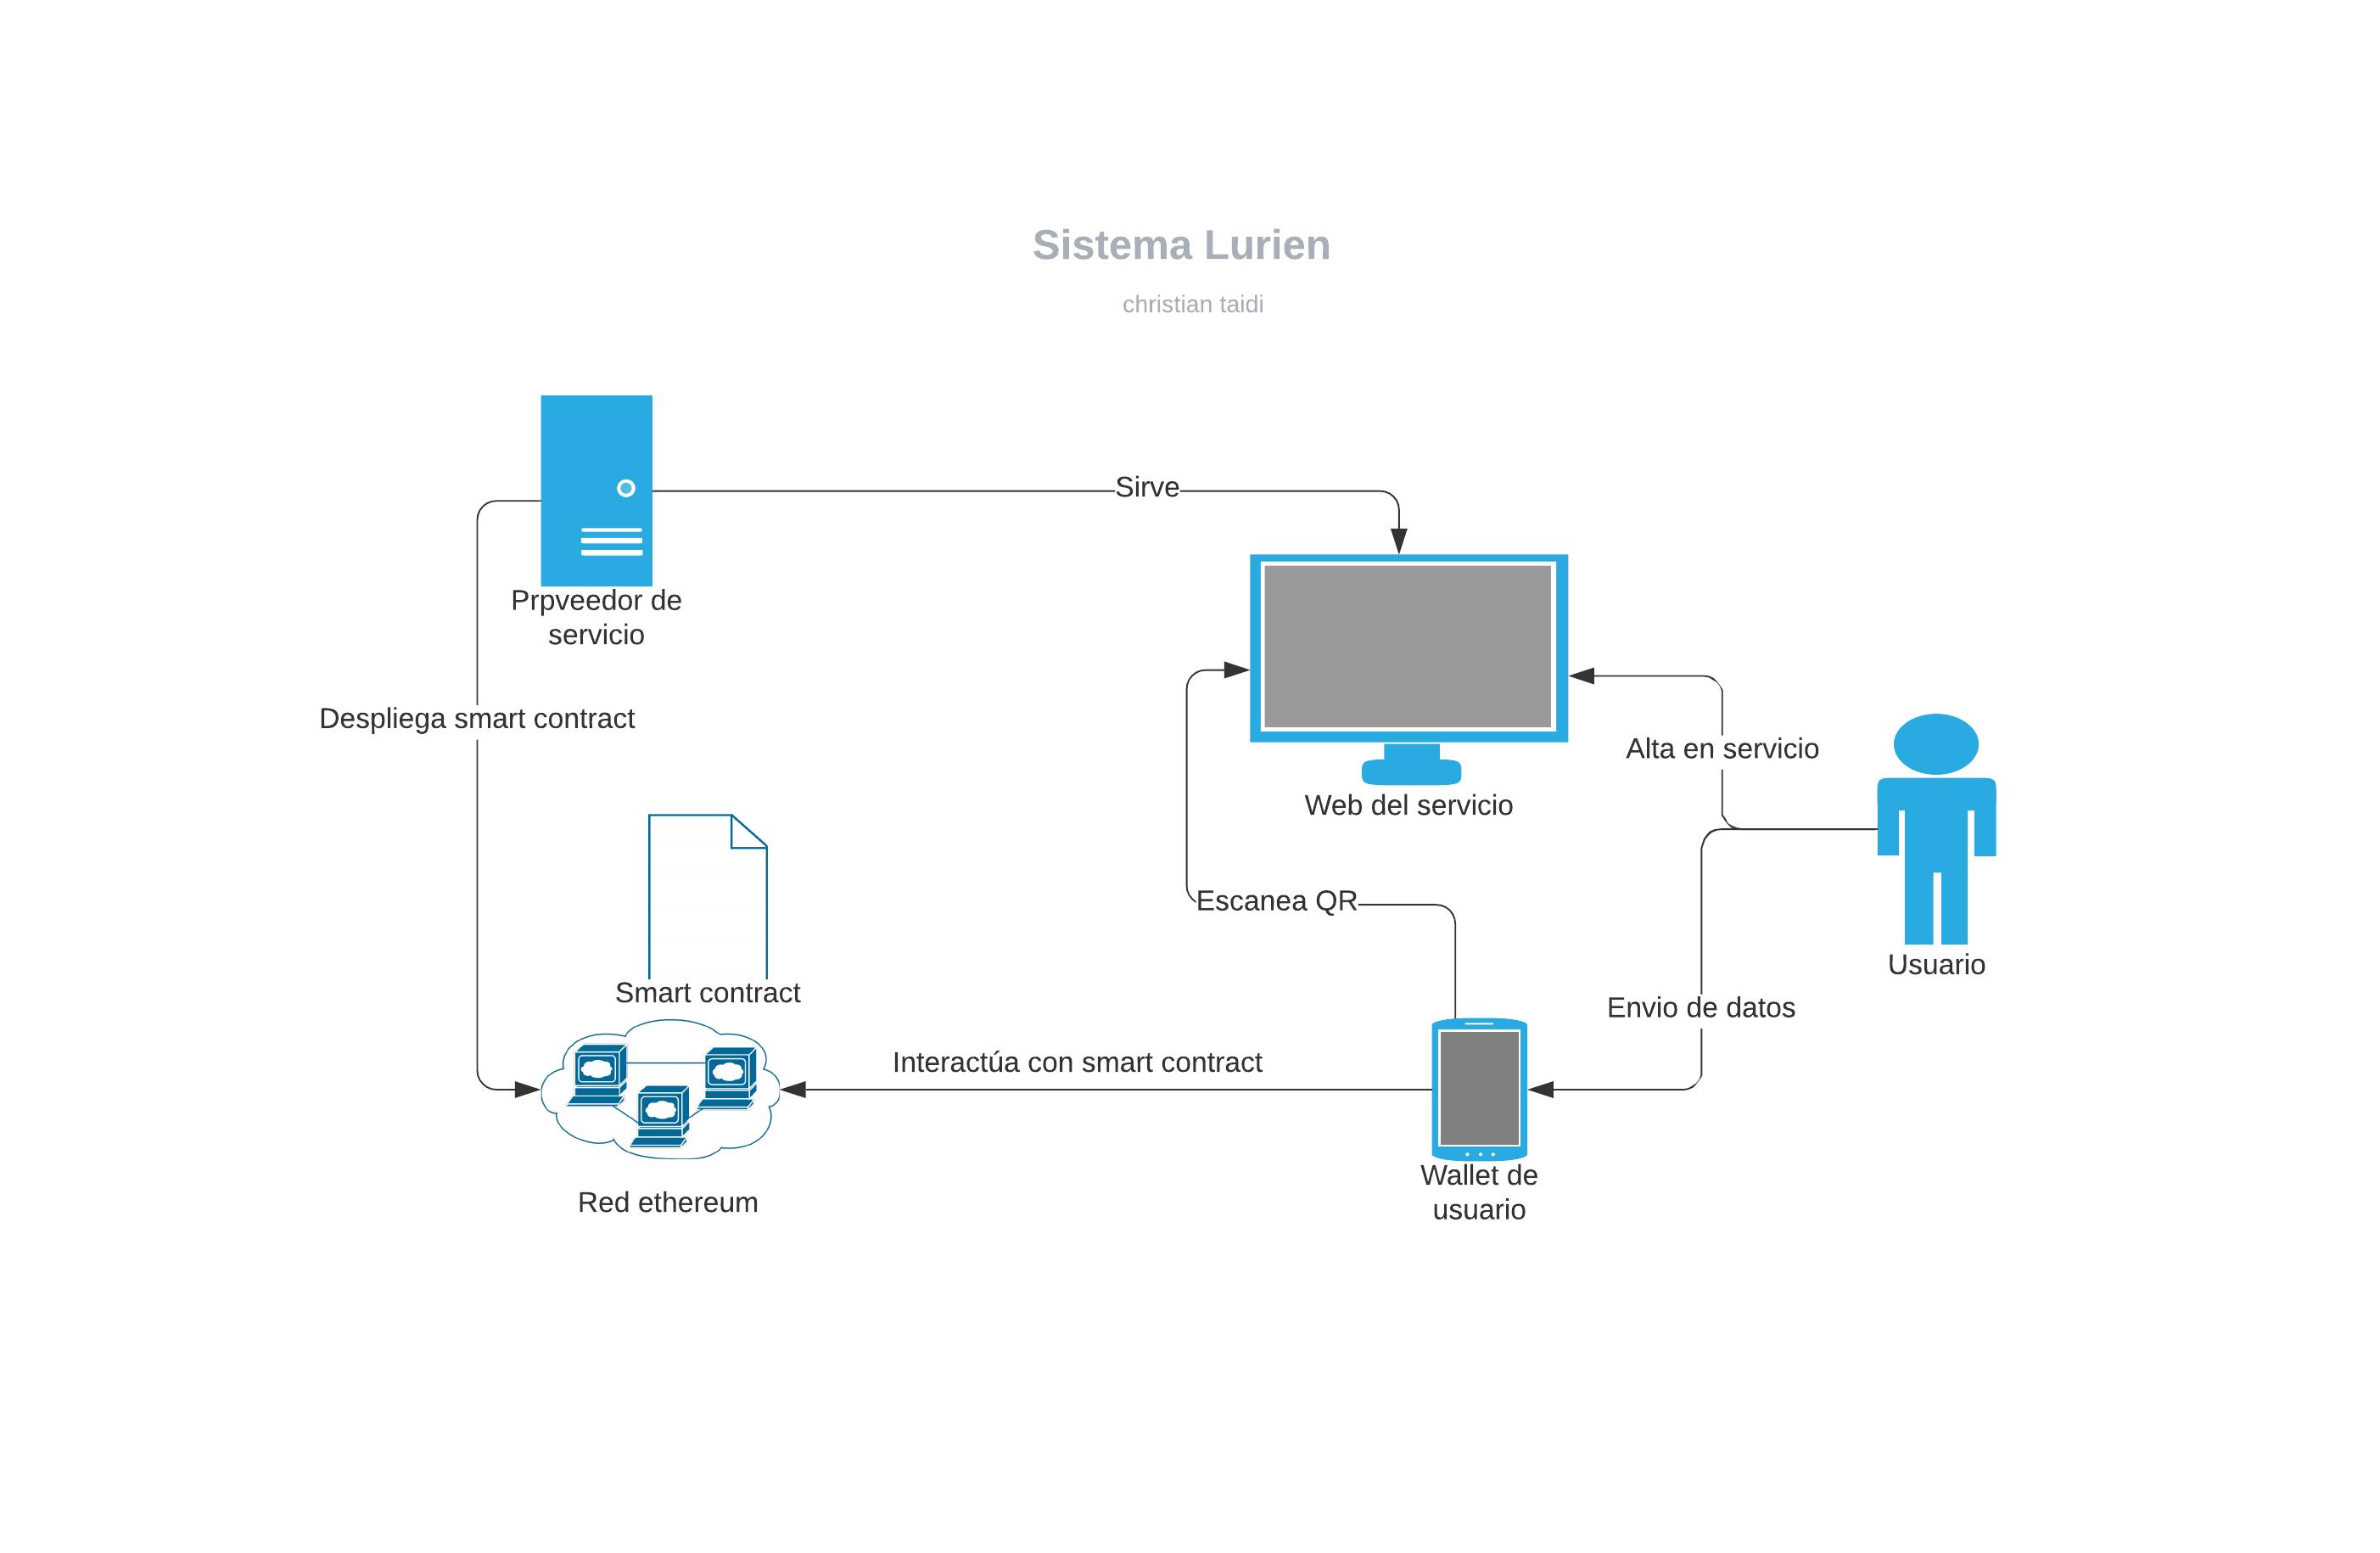
\includegraphics[width=1\textwidth]{componentes}
\caption{Componentes principales del sistema y sus interacciónes}
\end{figure}
\section{Proceso}
El proceso propuesto intenta simplificar la transmisión de los datos solicitados por el servicio y facilitar al proveedor de servicio un registro inmutable que recoja la transacción de datos sin almacenar dichos datos.

Para comenzar el proceso necesitamos asumir ciertas cosas que no han sido implementadas por complejidad.
\begin{enumerate}
\item El CA ha emitido y firmado digitalmente el assert correspondiente con el DNI al Wallet de usuario.
\item El usuario ya posee en su Wallet el assert correspondiente con su nota de selectividad y el pago de las tasas necesarias para realizar las pruebas de acceso.
\item El proveedor de servicio solo necesita el DNI del usuario, su nombre, su correo electrónico, su nota de selectividad y el certificado de haber pagado las tasas correspondientes a la prueba de acceso.
\item Los datos transmitidos a traves del smart contract estan cifrados mediante una clave asimétrica utilizando la clave pública del proveedor de servicio.
\item Los datos transmitidos están firmados digitalmente por el usuario de modo que el proveedor de servicio verifica que proceden de quien dice ser.
\item La red Ethereum utilizada es privada y está configurada para que los usuarios tengan fondos iniciales para poder hacer transacciones a través del smart contract.

\item El smart contract utilizado expone una interfaz común a todos los smart contract utilizados para este proceso por cualquier otro proveedor de servicio, de forma que el Wallet pueda realizar transacciones con cualquier smart contract de cualquier proveedor a través de las mismas funciones genéricas.
\item El proveedor de servicio almacena los datos del usuario en su base de datos de clientes y notifica al usuario de su alta mediante un correo electrónico tras terminar el proceso.

\end{enumerate}
 
Para comenzar el proceso el usuario deberá buscar la página web del proveedor de servicio en el que quiere darse de alta y seleccionar la opciópn de registro.

Al recibir la petición de alta, el proveedor de servicio desplegará una instancia de su smart contract en la red Ethereum y obtendrá la dirección del contrato desplegado generando un código QR con esa dirección y quedandose a la escucha de un evento emitido por el smart contract cuando el usuario transmita su información.

El usuario deberá escanear el código QR generado por el proveedor con su Wallet, lo que hará una consulta al smart contract para conocer los datos que se necesitan para darse de alta, en este caso el DNI, el nombre,la dirección de correo electrónico, la nota de selectividad y el certificado de haber pagado las tasas necesarias.

Después de que el Wallet haya recibido la respuesta del contrato, mostrará al usuario los datos que se piden y este deberá aceptar o no compartir esos datos con el servicio.

Al aceptar la transmisión de los datos, el Wallet realiza una llamada a una función del contrato con los datos solicitados disparando el evento al que está suscrito el proveedor de servicio.

El proveedor de servicio recibe los datos, los valida y verifica utilizando la firma digital del usuario y del CA.

Todo el intercambio de datos se almacena en la blockchain como una serie de transacciónes con un smart contract que tiene como datos la dirección del smart contract y las direcciones del usuario y del proveedor de servicio.

\section{Requisitos}
En esta sección se exponen los requisitos de cada elemento que compone el sistema con el objetivo de definir el funcionamiento del software a desarrollar de forma precisa y ordenada, además de algunos requisitos no funcionales que afectan a la usabilidad y robustez del sistema.


 
\begin{description}
\item[Universidad Rey Juan Carlos (Service Provider)]\
	\begin{itemize}
	\item[\textbf{RF.1}] El proveedor de servicio expondrá una interfaz web para que el 		usuario interactúe con él.
	\item[\textbf{RF.2}] El proveedor de servicio desplegará una instancia de su smart 		contract cada vez que un usuario solicite darse de alta en el sistema.
	\item[\textbf{RF.3}] El proveedor de servicio se encargará de comprobar la firma 		digital de los datos recibidos y notificar en caso de que los datos no 		sean completos o correctos.
	\item[\textbf{RF.4}] El proveedor de servicio mantendrá un estado de escucha tanto a 	la interfaz web como a los eventos del smart contract.
	\end{itemize}
\end{description}

\begin{description}
\item[Wallet de usuario]\
	\begin{itemize}
	\item[\textbf{RF.1}]El wallet de usuario almacenará todos los asserts correspondientes al usuario.
	\item[\textbf{RF.2}]El wallet de usuario realizará escaneos de códigos QR.
	\item[\textbf{RF.3}]El wallet de usuario utilizará un sistema de clave asimétrica para firmar los datos emitidos.
	\item[\textbf{RF.4}]El wallet de usuario mostrará al usuario la información del wallet y de los asserts almacenados.
	\end{itemize}
\end{description}

\begin{description}
\item[Smart contract]\
	\begin{itemize}
	\item[\textbf{RF.1}]El smart contract expondrá funciones públicas para que los usuarios puedan interactuar con él.
	\item[\textbf{RF.2}]El smart contract no almacenará ningún dato identificativo.
	\item[\textbf{RF.3}]El smart contract guardará la dirección del proveedor de servicio y la dirección del Wallet de usuario.
	\item[\textbf{RF.4}]El smart contract contendrá información acerca de los datos que requiere el proveedor de servicio.
	
	\end{itemize}
\end{description}

\begin{description}
\item[Red Ethereum]\
	\begin{itemize}
	\item[\textbf{RF.1}]La red Ethereum generará cuentas iniciales con fondos para poder realizar las transacciones.
	\item[\textbf{RF.2}]La red Ethereum establecerá unos parámetros de límite y coste de gas suficientes para poder desplegar y operar con el smart contract.
	
	\end{itemize}
\end{description}

\begin{description}
\item[Requisitos no funcionales]\
	\begin{itemize}
	\item[\textbf{RNF.1}]El wallet de usuario implementará un acceso autenticado mediante el uso de correo electrónico y contraseña.
	\item[\textbf{RNF.2}]El smart contract tendrá una baja carga computacional para reducir el coste de las transacciones.
	\item[\textbf{RNF.3}]El service provider tendrá una buena conexión a internet para desplegar el smart contract en menos de 4 segundos.
	\item[\textbf{RNF.4}]El wallet de usuario tardará menos de 5 segundos en obtener y mostrar la información necesaria para el service provider.
	\item[\textbf{RNF.5}]La red Ethereum será accesible tanto por el proveedor de servicio como por el Wallet de usuario para permitir la comunicación.
	\end{itemize}
\end{description}

\section{Prototipo}
En este apartado se explican los pasos llevados a cabo para desarrollar el sistema completo utilizado para el caso de uso, separando cada subsistema y concluyendo con la integración entre ellos.

\subsection{Service Provider}
Este sistema ha sido desarrollado en Java como un servicio web, utilizando el framework Spring para facilitar las comunicaciones mediante el protocolo HTTP tanto con la interfaz web como con el smart contract en Ethereum.
Para poder ejecutar el código es necesario tener una red blockchain local en el puerto 7545 para poder realizar la conexión. 
\begin{description}
\item Requisitos previos:
	\begin{itemize}
	\item Java 8 o superior.
	\item Una red ethereum local en el puerto 7545 o remota utilizando el nodo de Infura (En caso de utilizar una red remota modificar el archivo application.properties) .
	\item Maven.
	\end{itemize}
\end{description}

Para replicar el caso de uso es necesario realizar los siguientes pasos:

\begin{enumerate}
\item Clonar el repositorio del proyecto \href{https://github.com/ChristianTaidi/LurienServicePRovider}{Lurien Service Provider}.
\item Ejecutar los comandos \textit{mvn install} y \textit{mvn package}.
\begin{figure}{H}
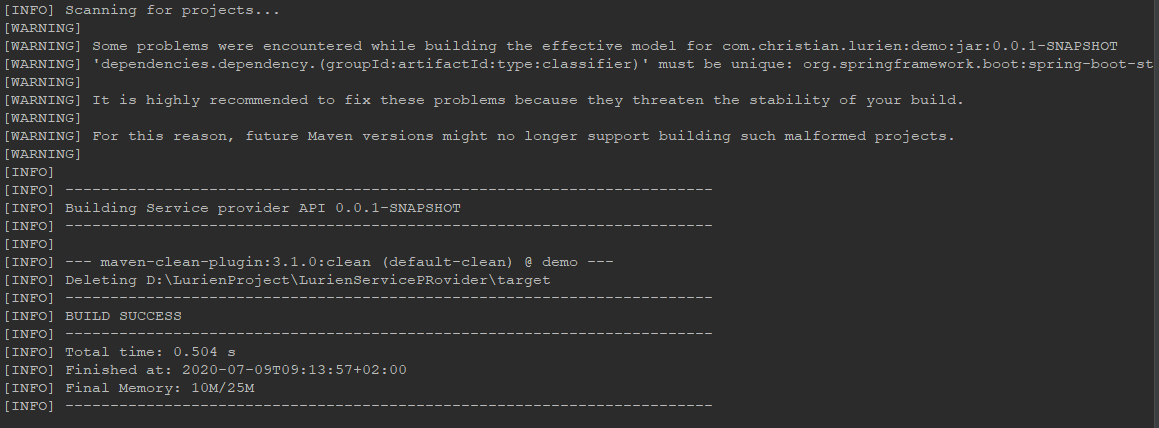
\includegraphics[width=1\textwidth]{mvn-clean}
\caption{Resultado de ejecutar mvn clean install}
\end{figure}

\begin{figure}{H}
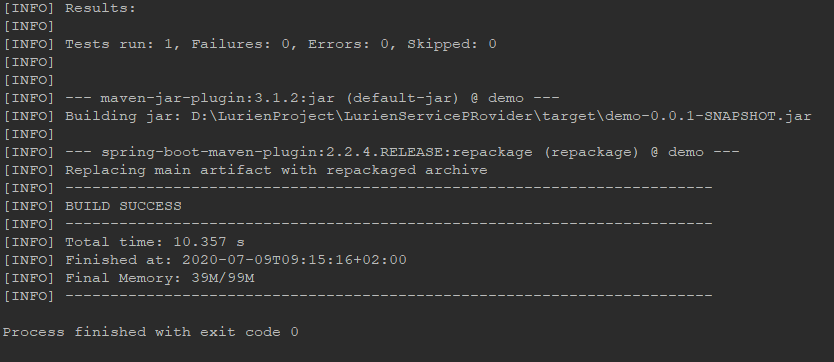
\includegraphics[width=1\textwidth]{mvn-package-result}
\caption{Resultado de ejecutar mvn package }
\end{figure}

\item Ir a la carpeta \textit{target} y ejecutar el comando \textit{java -jar demo-0.0.1-SNAPSHOT.jar}.
\item Buscar en el navegador la dirección y el puerto del servicio web para poder ver la página localhost:8443.
\end{enumerate}

\subsection{Wallet de usuario}
El wallet de usuario es una aplicación móvil que se ha desarrollado en Java utilizando Android Studio como entorno de desarrollo para facilitar el diseño de las interfaces gráficas de la aplicación. La aplicación utiliza permisos de almacenamiento, cámara e internet.

La autenticación de la aplicación está implementado utilizando Firebase para simplificar la gestion de cuentas y contraseñas.

\begin{description}
\item Requisitos previos:
	\begin{itemize}
	\item Java 8 o superior.
	\item Gradle.
	\item Compilador de Android 10(Api 29).
	\item Android Studio.
	\item Conexión a internet para acceder a Firebase.
	\end{itemize}
\end{description}

Para replicar el caso de uso es necesario realizar los siguientes pasos: 
\begin{enumerate}
\item Clonar el repositorio del proyecto \href{https://github.com/ChristianTaidi/LurienWallet}{Lurien Wallet}.
\item Configurar la version de android y del compilador.

\item Conectar el teléfono Android en modo desarrollador al ordenador.

\item Permitir la depuración en el teléfono.
\begin{figure}[H]
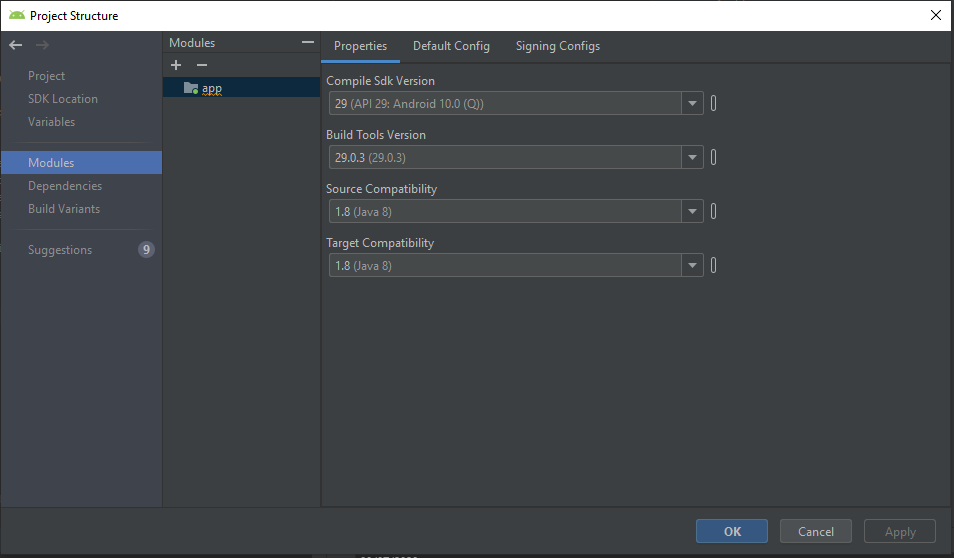
\includegraphics[width=1\textwidth]{config-android}
\caption{Configuración de versión de android y versión de java}
\end{figure}
\begin{figure}[H]
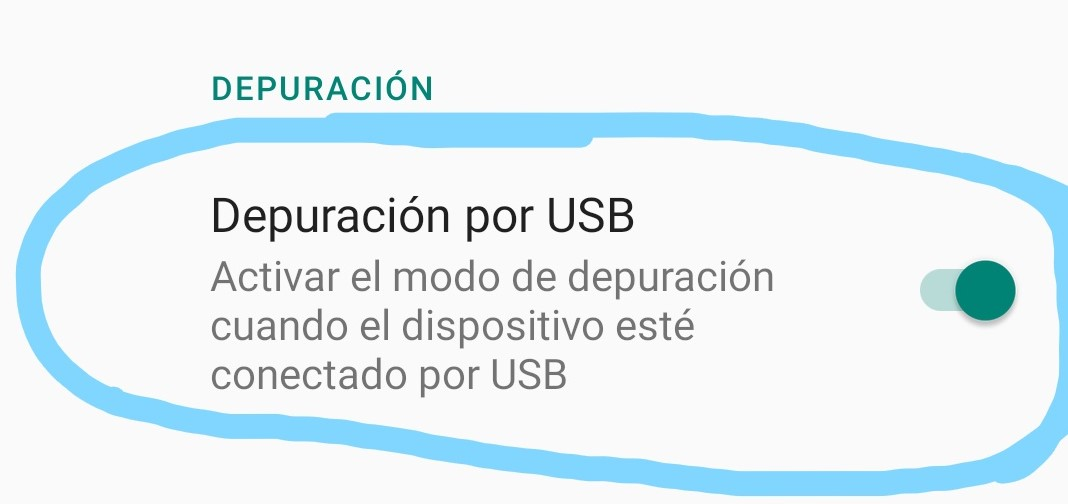
\includegraphics[width=0.7\textwidth]{debug-android}
\caption{Activar depuración por USB}
\end{figure}

\item Seleccionar el teléfono como entorno de ejecución en Android Studio .
\item Ejecutar el código para instalar la aplicación en el teléfono.
\item Ejecutar la aplicación en el teléfono.
\item Crear una cuenta de usuario con un correo electrónico y una contraseña.
\begin{figure}[H]
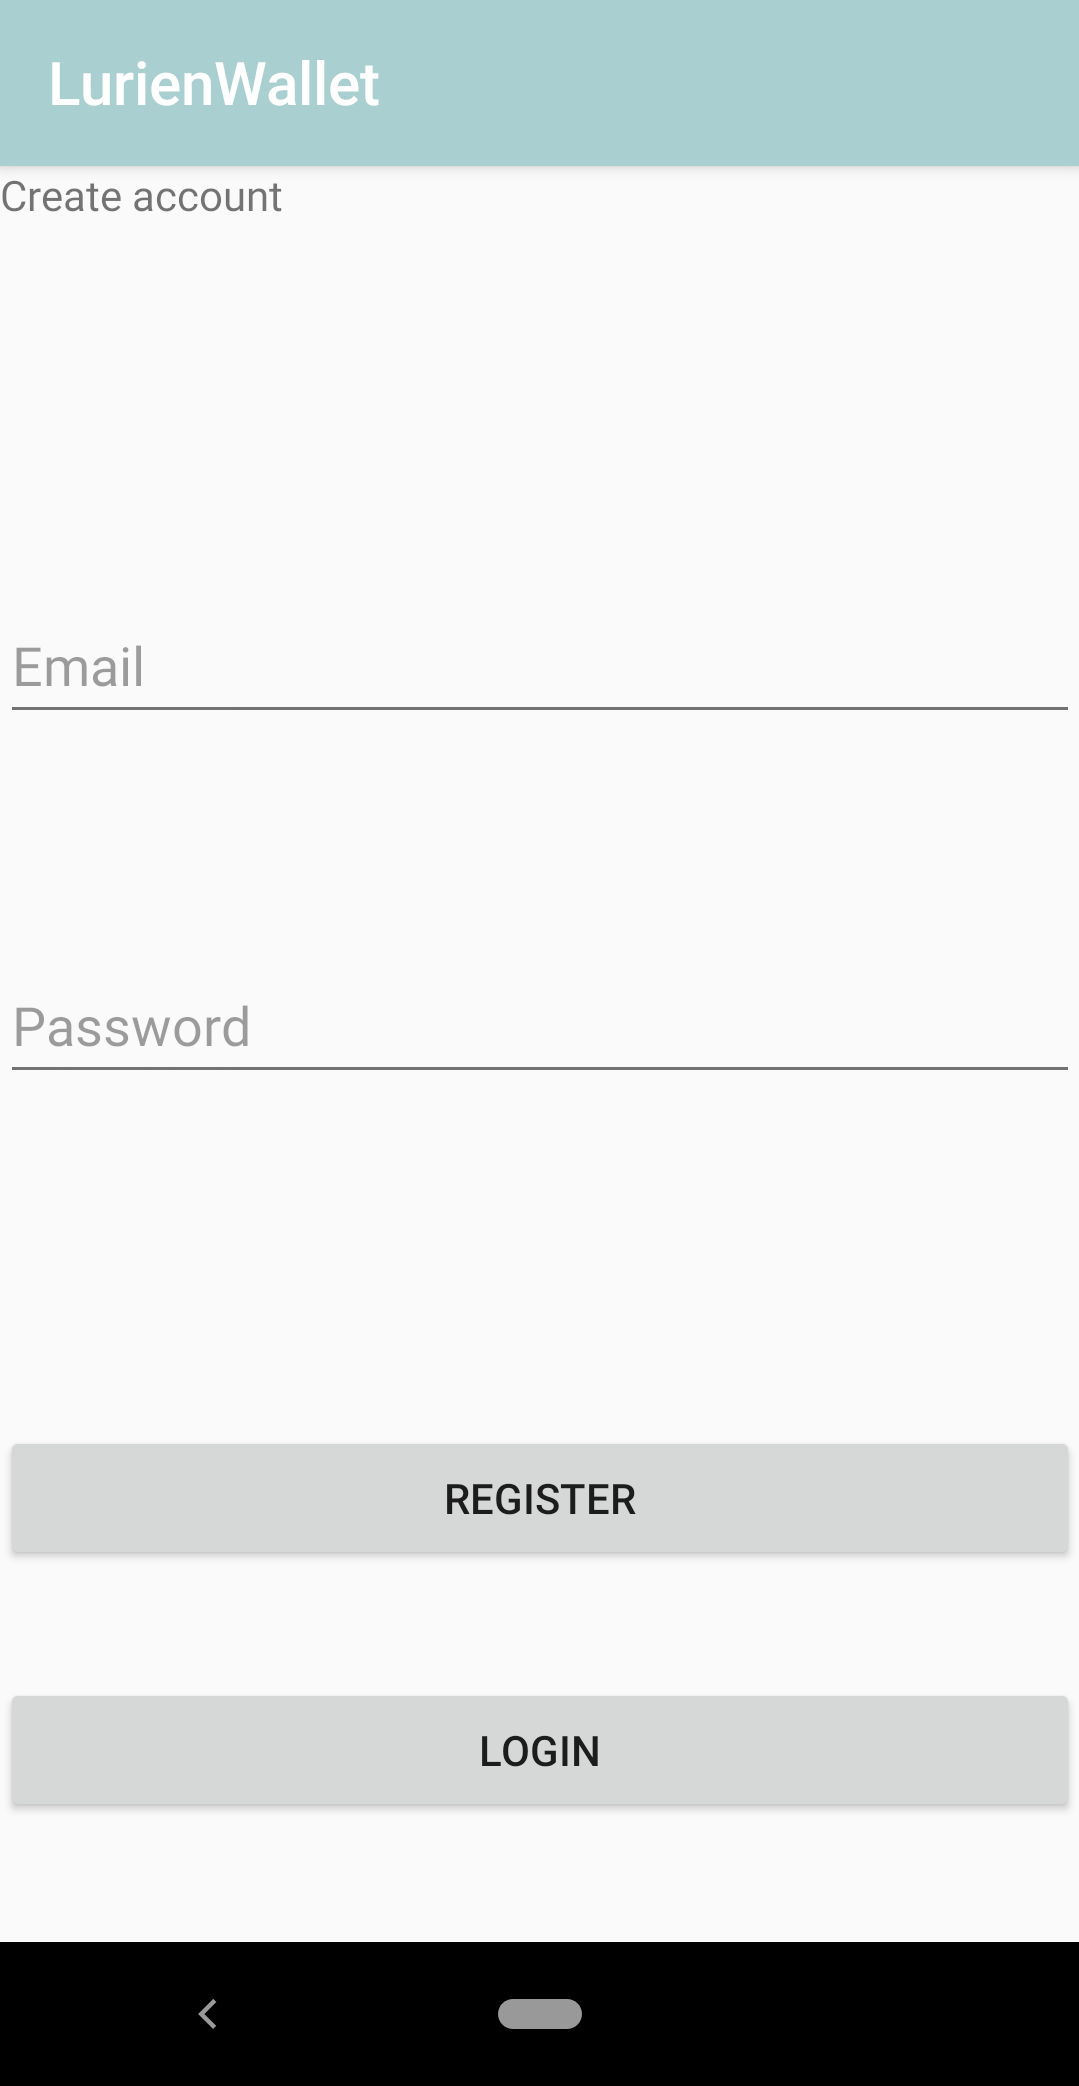
\includegraphics[width=0.5\textwidth]{login-register}
\caption{Pantalla de registro/inicio de sesión}
\end{figure}

\item Iniciar sesión.
\item Si el Service Provider está activo el usuario deberá acceder a su página web y seleccionar la opción darse de alta.
\begin{figure}[H]
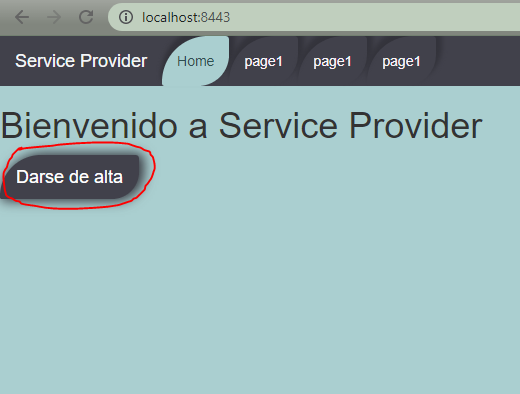
\includegraphics[width=0.8\textwidth]{service-provider}
\caption{Página principal del proveedor de servicio}
\end{figure}

\item En el Wallet pulsar el botón para escanear código QR.
\begin{figure}[H]
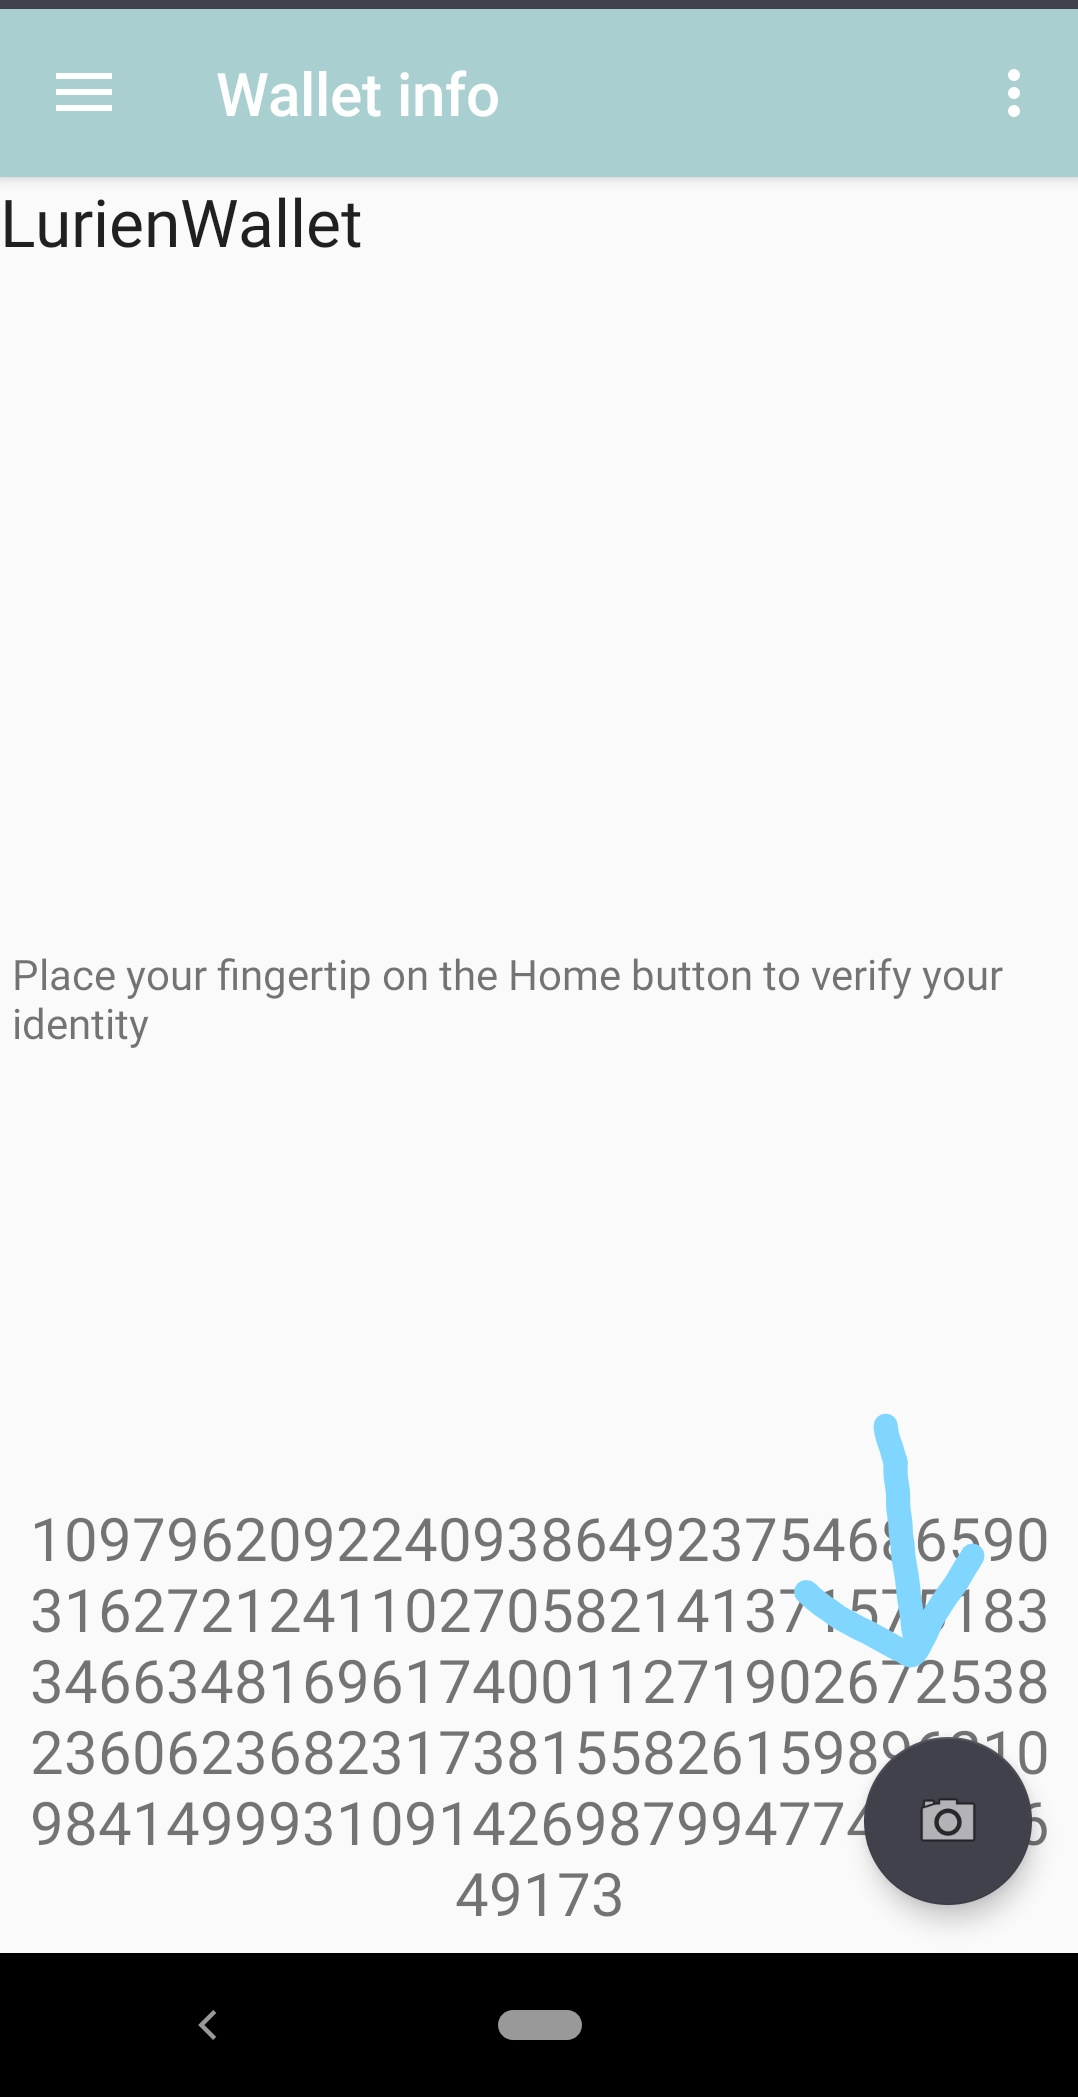
\includegraphics[width=0.5\textwidth]{main-screen}
\caption{Pantalla principal de la aplicación}
\end{figure}

\item Enfocar el código QR mostrado en la página web para escanearlo.
\begin{figure}[H]
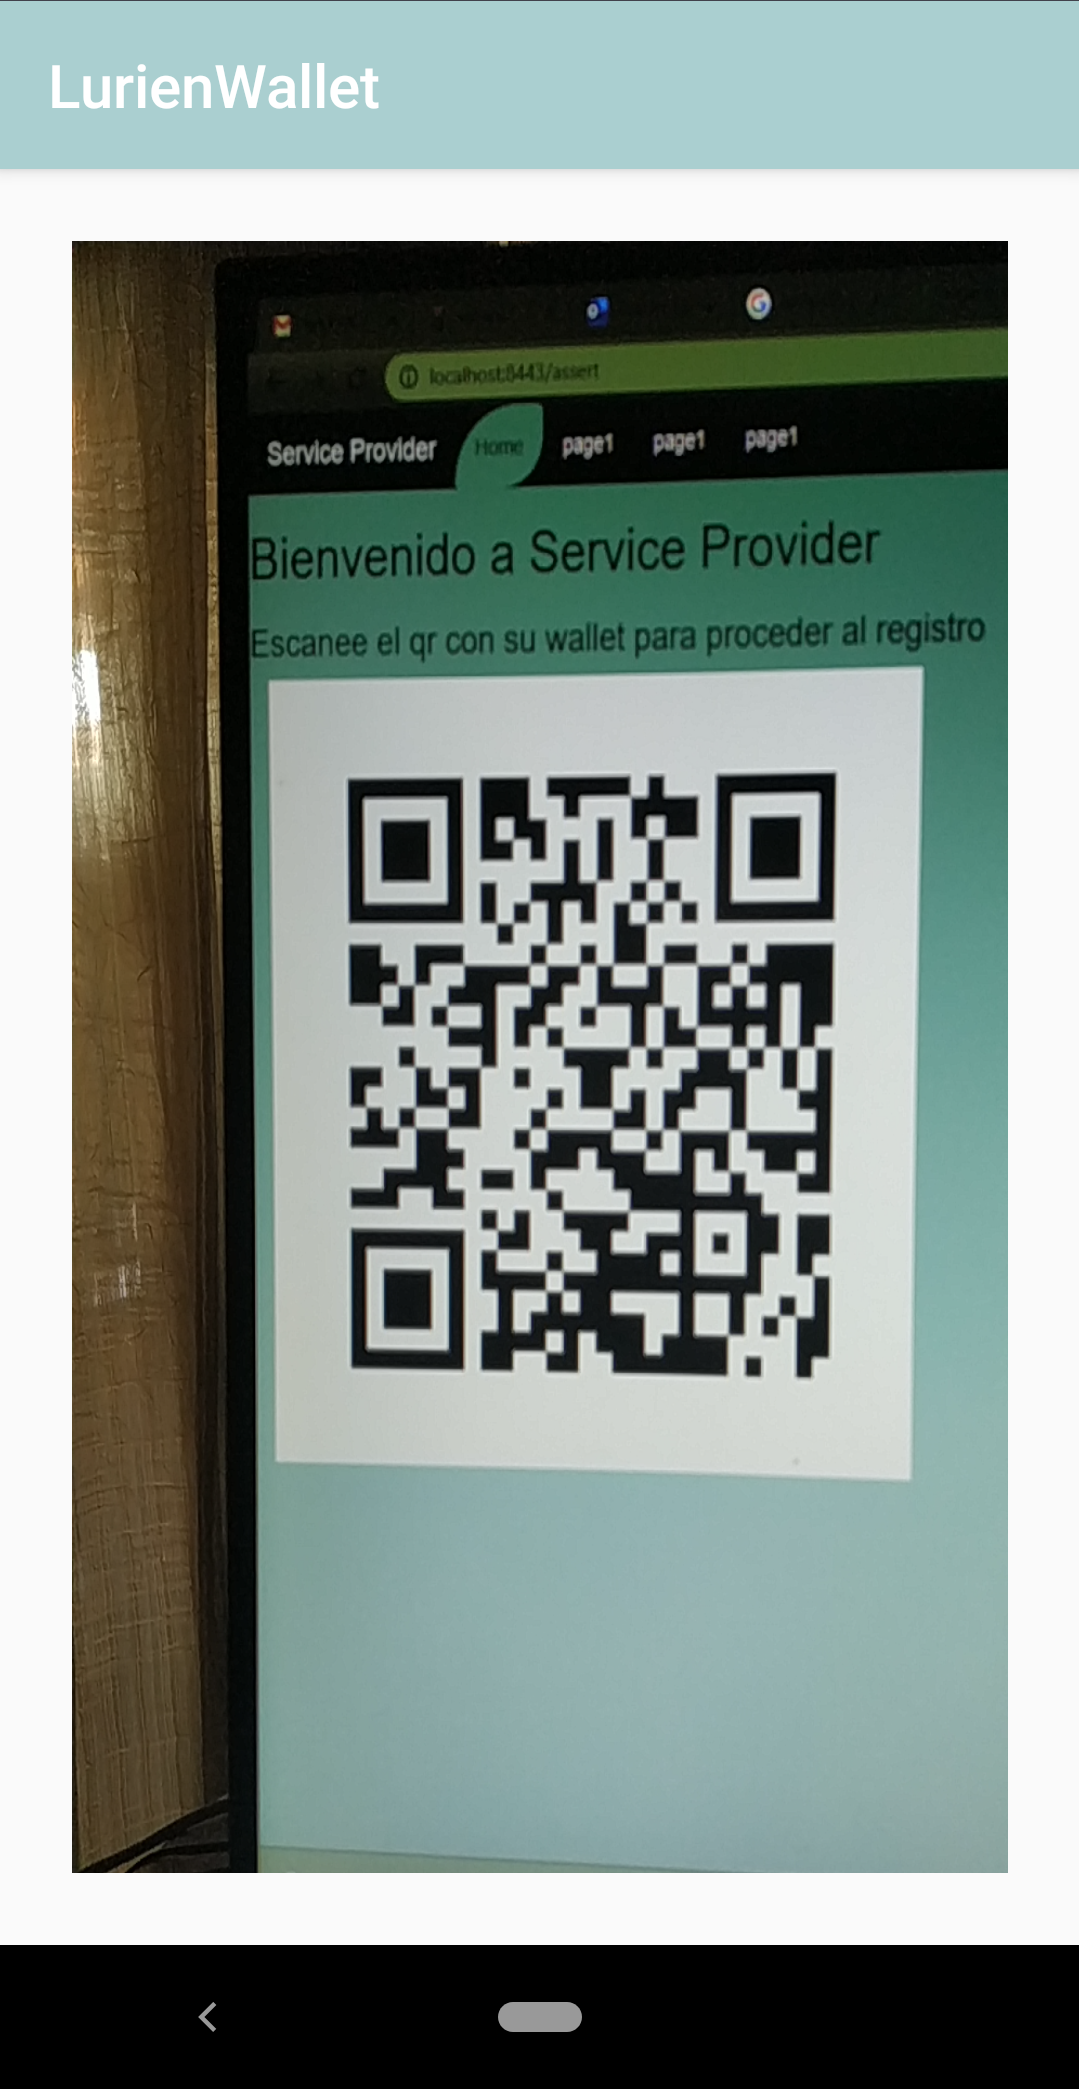
\includegraphics[width=0.5\textwidth]{qr-scan}
\caption{Escaneo de código QR con la aplicación}
\end{figure}

\item Esperar a que se muestren los datos que solicita el servicio.
\begin{figure}[H]
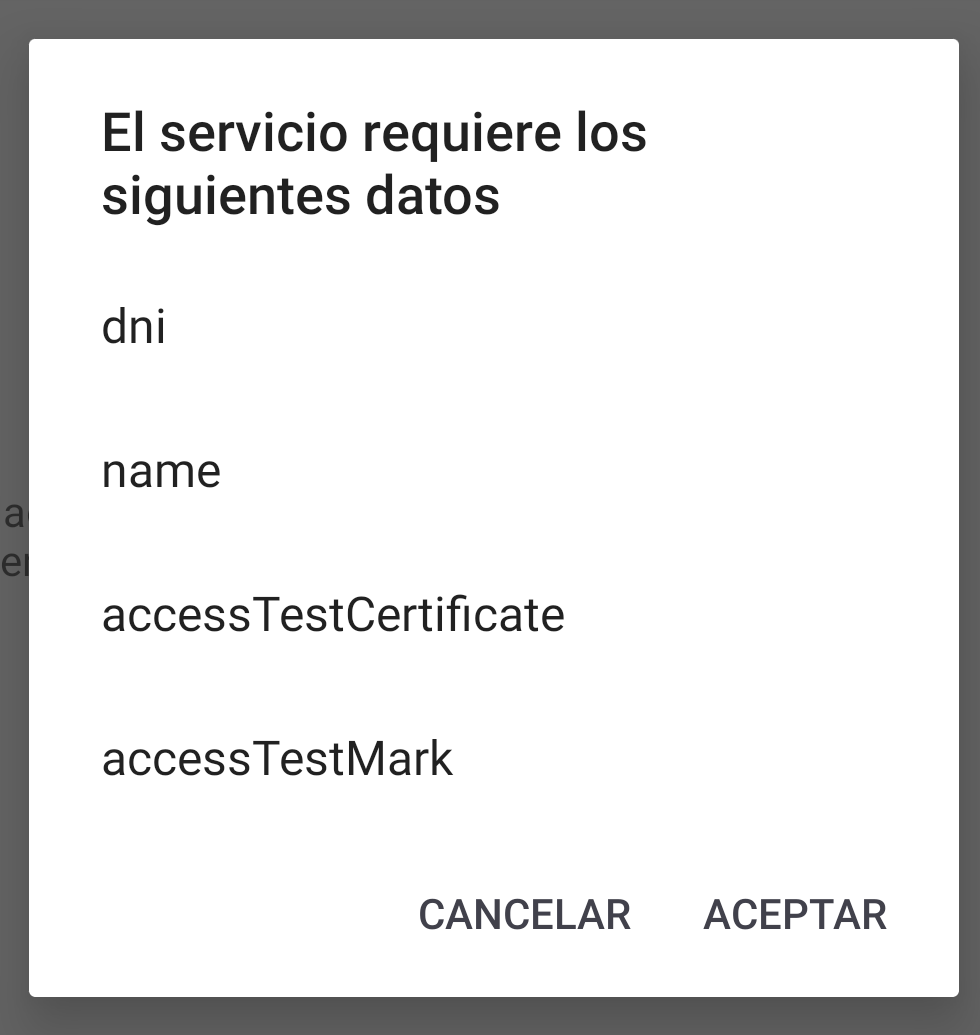
\includegraphics[width=0.5\textwidth]{data-required}
\caption{Datos requeridos por el proveedor de servicio}
\end{figure}

\item El usuario debe aceptar compartir los datos para enviarlos al proveedor de servicio y darse de alta. En caso de que no acepte no se realizará el alta en el servicio.
\end{enumerate}

\
\subsection{Smart contract}
El smart contract ha sido desarrollado en solidity 0.6.1 ya que las versiones anteriores no soportaban ciertas funcionalidades necesarias para el subsistema. Como soporte he utilizado el entorno de desarrollo Remix para probar que las distintas funcionalidades cumplian las especificaciones antes de integrarlo en el sistema.

\begin{description}
\item Requisitos previos:
	\begin{itemize}
	\item Web3j o una máquina virtual que tenga instalado web3j.
	\item Docker o solc para compilar el smart contract.
	\item Máquina virtual Ubuntu en caso de utilizar Docker y web3j en linux.
	\end{itemize}
\end{description}

Para compilar el smart contract y obtener el código java utilizado por el wallet y el service provider, es necesario realizar los siguientes pasos:
\begin{enumerate}
\item Clonar el repositorio del proyecto \href{https://github.com/ChristianTaidi/LurienSmartContracts}{Lurien Smart Contracts}.
\item Entrar en la carpeta LurienSmartContracts.
\item Ejecutar \textit{docker run --rm -v '<ruta a la carpeta contracts del proyecto>':'/contracts' -w '/contracts' ethereum/solc:0.6.1 '/contracts/LurienContract.sol' --bin --abi --optimize -o '/contracts' --overwrite} para compilar el contrato generando un archivo .bin y un archivo .abi. 

\begin{figure}[H]
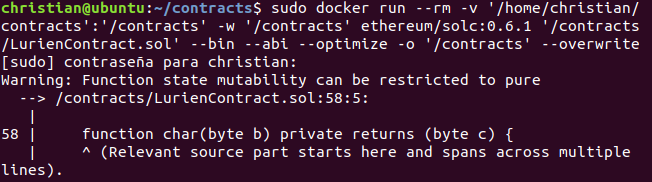
\includegraphics[width=0.8\textwidth]{smart-contract-compile}
\caption{Resultado de la compilación del smart contract}
\end{figure}

\begin{figure}[H]
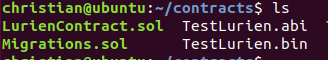
\includegraphics[width=0.8\textwidth]{compiled-contracts}
\caption{Archivos .abi y .bin generados tras la compilación}
\end{figure}
\item Generar la interfaz Java para interactuar desde el service provider y desde el Wallet utilizando web3j 'web3j solidity generate --binFile=TestLurien.bin --abiFile=TestLurien.abi -p contract.model -o src/main/java/'.

\begin{figure}[H]
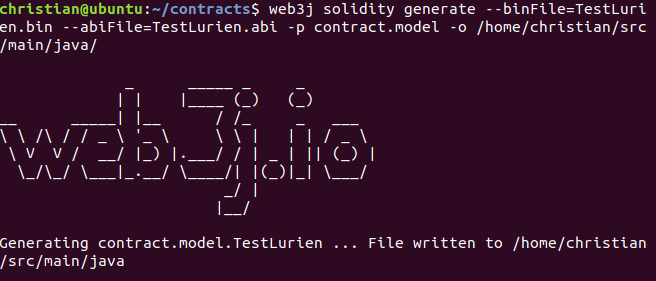
\includegraphics[width=0.8\textwidth]{smartcontract-java}
\caption{Resultado de ejecutar el comando web3j solidity generate}
\end{figure}

\begin{figure}[H]
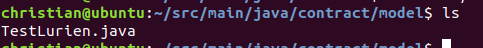
\includegraphics[width=0.8\textwidth]{built-java}
\caption{Archivo .java generado tras ejecutar el comando}
\end{figure}

\item Añadir el archivo .java a los paquetes de los subsistemas service provider y wallet.

\end{enumerate} 

Estos pasos deberán realizarse si se modificara en algún momento el código del smart contract, si no no es necesario ya que la interfaz java se encuentra en los proyectos del proveedor de servicio y del wallet de usuario.

\subsection{Red Ethereum}
La red Ethereum se ha creado en un principio en Ubuntu pero posteriormente en Windows ya que en el proceso he encontrado herramientas muy útiles que podrían utilizarse en un sistema Windows con facilidad.
 

\begin{description}
\item Requisitos previos:
	\begin{itemize}
	\item Truffle v5.1.14 (En caso de utilizar una red local).
	\item Ganache v2.4.0 (En caso de utilizar una red local).
	\item Un nodo en Infura ya sea para la red Rinkeby o Ropstein (En caso de utilizar una red remota).
	\item Haber clonado el repositorio LurienSmartContracts.
	\end{itemize}
\end{description} 
 
Aunque se indican requisitos para poder utilizar una red Ethereum remota, el proyecto está configurado para funcionar en una red local lo que permite realizar más transacciones al tener la capacidad de configurar las cuentas iniciales de la red. 
 
La red Ethereum se puede inciar de varias formas la más sencilla es utilizando Ganache:
\begin{enumerate}
\item Ejecutar Ganache.

\begin{figure}[H]
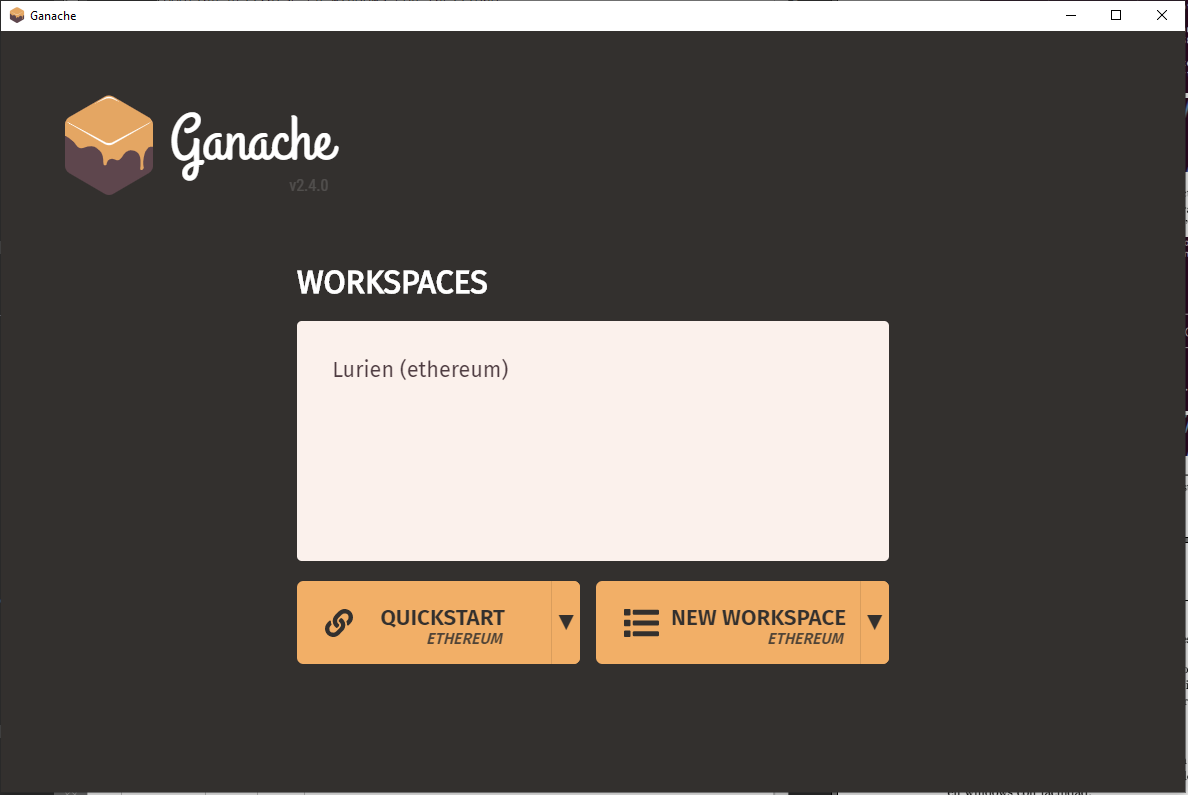
\includegraphics[width=0.8\textwidth]{ganache-ini}
\caption{Pantalla de inicio de Ganache}
\end{figure}


\item Modificar el archivo truffle.config para configurar los parámetros de la red si es necesario.

\begin{figure}{H}
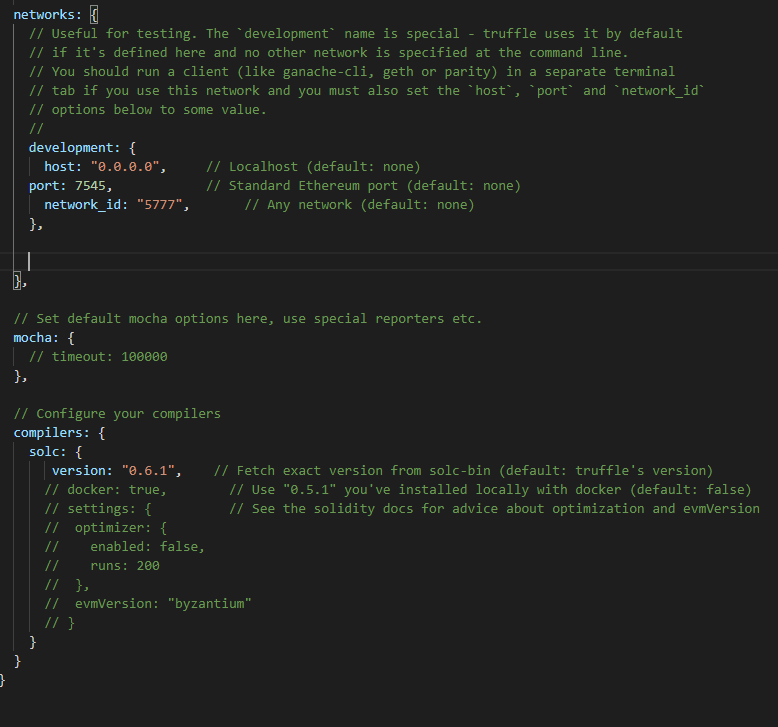
\includegraphics[width=0.8\textwidth]{truffle-configjs}
\caption{Archivo de configuración de la red blockchain}
\end{figure}

\item Crear un nuevo espacio de trabajo y seleccionar el archivo truffle-config del proyecto.

\begin{figure}{H}
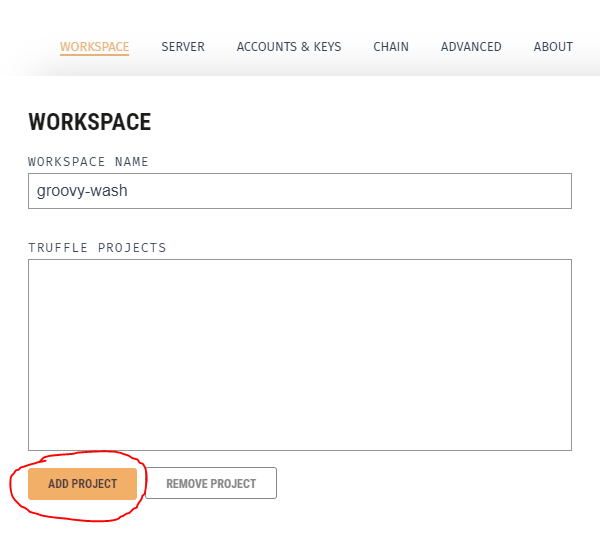
\includegraphics[width=0.8\textwidth]{ganache-addtruffle}
\caption{Cargar el archivo de configuración a Ganache}
\end{figure}

\begin{figure}{H}
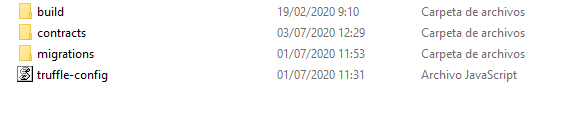
\includegraphics[width=0.8\textwidth]{truffle-config}
\caption{Archivo de configuración de truffle en el repositorio}
\end{figure}

\item Cambiar la configuración de servidor seleccionando como hostname todas las interfaces (0.0.0.0).

\item Guardar la configuración el espacio de trabajo e iniciar la red.

\item Al iniciar de nuevo ganache se mostraran los espacios de trabajo configurados previamente, seleccionar el generado con la configuración indicada.

\end{enumerate}
\chapter{Conclusiones}
En este trabajo se ha propuesto y analizado un uso alternativo de la tecnología blockchain aprovechando sus cualidades de inmutabilidad, integridad y no repudio para mantener un registro de las transacciónes de datos entre un usuario y un proveedor de servicio. Aunque el ámbito del concepto tras el trabajo es el entorno financiero y el blanqueo de capitales, es útil en cualquier tipo de proceso de alta en un servicio, ya que se necesita en cualquier caso mantener un registro del proceso en caso de posteriores consultas.
\section{Problemas encontrados}
\subsection{Dudas iniciales para enfocar el caso de uso}
Al principio del proyecto el enfoque del trabajo era el uso de la tecnología blockchain como medio para alcanzar la identidad auto-soberana, pero tras diversos debates y reflexiones determiné que debido a la regulación en materia de protección de datos, almacenar datos de usuario en un registro inmutable vulneraba el derecho al olvido del usuario ya que es imposible eliminar sus datos, estén o no encriptados, de la cadena. Por tanto decidí tomar un enfoque más transaccional llegando así al uso de la tecnología blockchain, no para almacenar datos de usuario sino para registrar transacciones de datos entre un usuario y una entidad de forma que haya un respaldo persistente e inalterable para el proceso KYC de los proveedores de servicio. Al no saber demasiado acerca de este tema he necesitado mucho tiempo para informarme y leer además de generar momentos de incertidumbre a la hora de elegir como proceder en cada parte del desarrollo
.
\subsection{Desarrollo desde cero}
Para el desarrollo del prototipo inicial no contaba con ningún tipo de código existente aunque conocía algunas organizaciones que estaban trabajando en algo parecido, pero eso no me permitiría aprender todo lo necesario acerca del funcionamiento de la tecnología blockchain y la interacción de esta con el mundo real. Por tanto me ha tomado más tiempo el desarrollo pero a cambio he aprendido cómo funciona un ciclo completo de interacción no solo con una cadena sino también con un smart contract, desde una aplicación y un servicio web.
\subsection{Uso de Alastria}
A mitad del desarrollo comenzé a investigar acerca de Alastria, una de las organizaciones que se encarga de establecer convenios con distintos servicios y entidades para utilizar la tecnologia blockchain como registro de sus transacciones de datos. Por tanto decidí probar a utilizar los elementos ya desarrollados por ellos para aprovecharlos y quitar carga de trabajo, pero la falta de documentación y al no conocer por completo las tecnologías que usan, se me hizo muy difícil llegar a comprender cómo era el funcionamiento de los distintos sistemas que utilizan para poder realizar el proceso completo, lo que me hizo volver a mi prototipo creado desde cero.
\subsection{Muchos componentes interdependientes}
Al ser un ciclo completo de ejecución, intervienen muchos subsistemas para poder completar la tarea, y estos aunque están separados dependen unos de otros. Por ejemplo si el proveedor de servicio perdiese su conexión con la red Ethereum, no podría desplegar su smart contract lo que no permitiría al usuario darse de alta hasta que se recuperase la conexión, aunque el wallet funcionará perfectamente y podría darse de alta en otro servicio, pero a la hora de desarrollar el prototipo al utilizar un solo servicio, en el momento de encontrar un fallo de red, se hacía imposible realizar pruebas.

\subsection{Red remota e Infura}
Al desarrollar el prototipo, probé a utilizar una red existente aprovechando el servicio de Infura para conectarme a una testnet remota, pero para hacer pruebas de despliegue del smart contract y para interactuar con él es necesario tener fondos en \textit{Ether} ya que todas esas acciones tienen un coste en \textit{gas}. A pesar de haber creado una cuenta de Metamask y haber utilizado un \textit{faucet} de \textit{Ether} para conseguir fondos iniciales, solo podía utilizar la misma cuenta de Infura tanto para el service provider como para el wallet lo que daba como resultado una transacción entre dos entidades con la misma dirección en la red.

\section{Trabajo futuro}
Como he mencionado anteriormente aún falta mucho por avanzar en el desarrollo de este proyecto, los avances que se podrían hacer son los siguientes:

\begin{itemize}

\item Desarrollar una entidad de certificación que emita los asserts al wallet de usuario. Se desarrollaría un prototipo de entidad de certificación que generaría un tipo de assert firmándolo y transmitiendolo de forma segura al wallet, ya sea a través de un sistema de comunicación vía internet (correo electronico) ó de forma física escaneando el assert con el wallet.

\item Establecer un sistema de cifrado para la transmisión de los datos. De momento la transmisión de los datos a través del smart contract se realiza en claro. Por tanto cualquier sistema malicioso podría intentar un ataque man in the middle e interceptar la información emitida a través del smart contract, ya que utiliza el protocolo http.

\item Establecer un sistema de firma por parte del usuario. Los datos emitidos por el usuario se transmiten sin ningún tipo de firma digital, por lo que cualquier entidad maliciosa que diga ofrecer un servicio, podría utilizar los datos del usuario de forma fraudulenta intentando suplantar su identidad. Si el wallet del usuario firmase digitalmente los datos, al validar estos en cualquier servicio, si la firma no coincide con la clave pública del emisor, daría error siendo imposible que una entidad utilizara los datos firmados de un usuario.

\item Integración de una base de datos remota al wallet de usuario. De momento los datos de los asserts del usuario se almacenan en el teléfono, pudiendo así perderse todos los asserts en el momento en que el teléfono del usuario deje de funcionar. Al contar con una base de datos el usuario podría recuperar sus asserts en todo momento pudiendo así utilizar su cuenta en varios dispositivos distintos conteniendo la misma información.

\item Creación de usuarios de la red blockchain con fondos. En el prototipo, las cuentas de Ethereum utilizadas son las generadas al crear la red blockchain local y que tienen 100 unidades de Ether iniciales para realizar las transacciones. Como para poder interactuar con el smart contract se necesitan fondos y cada interacción tiene un coste, lo ideal sería configurar la red de forma que siempre que se de de alta una cuenta de Ethereum, se añadan unos fondos por defecto. Aunque lo ideal sería que el sistema fuese gratuito y al añadir unos fondos por defecto, se limita el número de transacciones aunque el coste sea ínfimo.

\item Notificar al usuario del alta en el servicio. De momento el servicio una vez recibe los datos, no notifica al usuario de haberlos recibido, por tanto no se sabe si ha fallado la comunicación entre el smart contract y el proveedor. Lo ideal sería añadir de forma remota al wallet del usuario el servicio al que se ha suscrito manteniendo de esta forma un registro de todos los servicios en los que se encuentra dado de alta. Para ello se utilizaría o bien el mismo smart contract, haciendo que el wallet esté a la espera de un evento, o una comunicación vía correo electrónico con un archivo que contenga la información del servicio y pueda incorporarse al wallet del usuario.
\end{itemize}




\printbibliography[
heading=bibintoc,
title={Bibliografía}
]


\end{document}